\appendix
\setcounter{lemma}{2}

\section*{Web Appendix A: Regularity conditions and proofs}
\setreflabel{A}
\label{app:proofs}

\subsection{A.1 Regularity conditions}

Throughout, $T$, $S$ and the cluster sizes are bounded, $G\to\infty$, and $C$ denotes a generic
finite constant. $\|\cdot\|$ is the Euclidean or Frobenius norm.

\begin{description}
\item[A4$'$ (local dependence).] Let $\mathcal C$ be the graph on clusters in which $g$ and $h$
are adjacent if $W_{ij}>0$ for some $i\in g$, $j\in h$, or if the policy rule of $g$ uses data
from $h$; its maximal degree is bounded. (i) The cluster primitives (unit effects and pre-sample
outcomes, weekly outcome innovations, weekly policy randomisation) are independent across
clusters, and the week-$t$ outcome innovations are independent of all primitives dated before
week $t$ and of the week-$t$ policy randomisation. (ii) $D_{gt}$ is a measurable function of the
week-$t$ policy randomisation of $g$ and of the histories before week $t$ of clusters within
distance $\rho$ of $g$ in $\mathcal C$; $Y_{gt}$ is a measurable function of the week-$t$ innovation
and unit effects of $g$ and of the outcomes before week $t$ and the week-$t$ policies of $g$ and
of the clusters adjacent to $g$.
\item[A6(i)] $\Theta=\Delta\times\mathcal B$ is compact, $\mathcal B\subset\mathbb R^2\times[0,\bar\Phi]$,
and $\theta_0$ is an interior point.
\item[A6(ii)] For all $i,t$: $\E\sup_\theta\|z_{it}\|^4|Y_{i,t+1}r_{it}(\theta)|^4\le C$,
$\E\|z_{it}\|^4Y_{it}{}^4\le C$, $\E\sup_\theta\|z_{it}\,\partial u_{it}(\theta)/\partial\theta^{\top}\|^2\le C$ and
$\E\sup_\theta\|z_{it}\otimes\partial^2u_{it}(\theta)/\partial\theta\partial\theta^{\top}\|^2\le C$. When the
instruments depend on a nuisance value $\eta$ (Lemma~\ref{lem:generated}), the same bounds hold
for $\partial z_{it}/\partial\eta$ and $\partial^2z_{it}/\partial\eta\partial\eta^{\top}$ uniformly in a
neighbourhood of $\eta^*$.
\item[A6(iii)] The limits as $G\to\infty$, $\bar g(\theta)=\lim G^{-1}\sum_g\E g_g(\theta)$ and
$\bar\Gamma(\theta)=\lim G^{-1}\sum_g\E\,\partial g_g(\theta)/\partial\theta^{\top}$ exist uniformly in
$\theta$; $\Gamma=\bar\Gamma(\theta_0)$; and
$\Sigma_s=\lim G^{-1}\sum_g\E(\xi_{gs}\xi_{gs}{}^{\top})$ exists for $s=1,\dots,T$.
\item[A6(iv)] $\Omega=\sum_s\Sigma_s$ is positive definite; $\Gamma$ has full column rank $p$;
$\bar g(\theta)^{\top}W\bar g(\theta)=0$ only at $\theta=\theta_0$.
\end{description}

\noindent Condition (L) collects the laws of large numbers. For every $\theta\in\Theta$,
$G^{-1}\sum_g\{f_g-\E f_g\}\to_p0$ for each of $f_g=g_g(\theta)$, $\partial g_g(\theta)/\partial\theta^{\top}$,
$g_g(\theta_0)g_g(\theta_0)^{\top}$, $\sup_\theta\|\partial g_g(\theta)/\partial\theta^{\top}\|$ and
$\sup_\theta\|\partial^2g_g(\theta)/\partial\theta\partial\theta^{\top}\|$; and, for $s=1,\dots,T$,
$V_s:=G^{-1}\sum_g\E(\xi_{gs}\xi_{gs}{}^{\top}\mid\F_{s-1})\to_p\Sigma_s$.

\noindent Lemma~\ref{lem:lln} shows that A4$'$ together with A6(ii)--(iii) implies (L). Under A4,
A6(ii) also implies the conditional Lyapunov condition of Lemma~\ref{lem:clt} with $\delta=1$:
$\E\{G^{-3/2}\sum_g\E(\|\xi_{gs}\|^3\mid\F_{s-1})\}\le CG^{-1/2}\to0$, so the conditional sum tends to
zero in probability by Markov's inequality.

\subsection{A.2 Proofs for Section~\ref{ss:moments}}

\begin{proof}[Proof of Lemma~\ref{lem:moment}]
Fix $t\ge1$ and a policy path $\mathbf d$. On the event $\{D_{1:t}=\mathbf d_{1:t}\}$, A3 and A2(a)
give $Y_{is}=Y_{is}(\mathbf d)$ for all $s\le t$, so $H_{t-1}=H_{t-1}(\mathbf d)$ and
$\Lambda_{it}=\Lambda_{it}(\mathbf d;\phi_0)$ there. Pre-sample outcomes do not depend on
$\mathbf d$ by A2(a), and $D=0$ before week 1. Because $D_{1:t}$ is discrete, A2(b) gives the following chain of equalities.
\begin{align*}
&\E(Y_{it}\mid\alpha,H_{t-1},D_{1:t}=\mathbf d_{1:t})\\
&\quad=\E\{Y_{it}(\mathbf d)\mid\alpha,H_{t-1}(\mathbf d),D_{1:t}=\mathbf d_{1:t}\}\\
&\quad=\E\{Y_{it}(\mathbf d)\mid\alpha,H_{t-1}(\mathbf d)\}
\end{align*}
The right side equals $e^{\alpha_i+\gamma_t+\tau_0d_{it}+\kappa_0\bar d_{it}}\Lambda_{it}(\mathbf d;\phi_0)$
by A1. Since $\F_{t-1}=\sigma(\alpha,H_{t-1},D_{1:t})$, this gives $\E(Y_{it}\mid\F_{t-1})=\mu_{it}$. Next,
$r_{it}=m_{it}(\theta_0)/m_{i,t+1}(\theta_0)$ depends on $D_{i,t+1}$, $\bar D_{i,t+1}$ and
$\Lambda_{i,t+1}$, all $\F_t$-measurable, and $r_{it}\mu_{i,t+1}=\mu_{it}$. Hence
$\E(u_{it}\mid\F_{t-1})=\E\{r_{it}\E(Y_{i,t+1}\mid\F_t)\mid\F_{t-1}\}-\mu_{it}=\mu_{it}-\mu_{it}=0$.
\end{proof}

\begin{proof}[Proof of Lemma~\ref{lem:mds}]
Since $r_{it}\mu_{i,t+1}=\mu_{it}$, $u_{it}(\theta_0)=r_{it}\varepsilon_{i,t+1}-\varepsilon_{it}$. Summing
$z_{it}u_{it}$ over $t=1,\dots,T-1$ and collecting the coefficient of each $\varepsilon_{is}$ gives
$g_g(\theta_0)=\sum_{s=1}^T\sum_{i\in g}a_{is}\varepsilon_{is}$ with $a_{is}$ as stated. Both
$z_{i,s-1}r_{i,s-1}$ and $z_{is}$ are $\F_{s-1}$-measurable. By Lemma~\ref{lem:moment},
$\E(\varepsilon_{is}\mid\F_{s-1})=0$, so $\E(\xi_{gs}\mid\F_{s-1})=0$ and $\xi_{gs}$ is $\F_s$-measurable.
For $s<s'$ and any clusters $g,h$,
$\E(\xi_{gs}\xi_{hs'}{}^{\top})=\E\{\xi_{gs}\E(\xi_{hs'}{}^{\top}\mid\F_{s'-1})\}=0$. This gives the first
claim with $g=h$. For $g\ne h$ and $s=s'$,
$\E(\xi_{gs}\xi_{hs}{}^{\top})=\sum_{i\in g,j\in h}\E\{a_{is}a_{js}{}^{\top}\E(\varepsilon_{is}\varepsilon_{js}\mid\F_{s-1})\}=0$,
because under A4 $\varepsilon_{is}$ and $\varepsilon_{js}$ are conditionally independent with
conditional mean zero.
\end{proof}

\begin{lemma}[Local law of large numbers]
\label{lem:lln}
Assume A4$'$ and let $L=(\rho+1)(T+1)+1$. If $f_g$ is a measurable function of the primitives of
the clusters within distance $L$ of $g$ in $\mathcal C$ and $\sup_g\E\|f_g\|^2\le C$, then
$G^{-1}\sum_g(f_g-\E f_g)\to_p0$. Each of the variables listed in (L) is of this form, so A4$'$
and A6(ii)--(iii) imply (L).
\end{lemma}

\begin{proof}
If the distance between $g$ and $h$ exceeds $2L$, then $f_g$ and $f_h$ are functions of
disjoint sets of primitives, which are independent by A4$'$(i), so $\cov(f_g,f_h)=0$. Let $B$
bound the number of clusters within distance $2L$ of any cluster; $B\le\sum_{k=0}^{2L}\Delta^k$
with $\Delta$ the maximal degree. Then
$\E\|G^{-1}\sum_g(f_g-\E f_g)\|^2\le G^{-2}\sum_g\sum_{h:\,d(g,h)\le2L}(\E\|f_g\|^2\E\|f_h\|^2)^{1/2}\le BC/G\to0$.

For locality, by A4$'$(ii) and induction on $t$, $(Y_{gt},D_{g,t+1})$ depends only on primitives of
clusters within distance $(\rho+1)(t+1)$ of $g$; the induction starts from pre-sample outcomes,
which are cluster primitives, and $D=0$ before week 1. The instruments $z_{it}$ use outcomes and
policies of $g$ and of adjacent clusters (through $N_{it}$ and $\bar D_{it}$), so $g_g(\theta)$ and
its derivatives depend on primitives within distance $L$. For the conditional variance, A4$'$
implies that, given $\F_{s-1}$, $Y_{gs}$ is a function of the week-$s$ innovation of $g$, which is
independent of $\F_{s-1}$, and of $\F_{s-1}$-measurable local quantities. Hence
$\E(\xi_{gs}\xi_{gs}{}^{\top}\mid\F_{s-1})$ is obtained by integrating out that innovation and is a
function of local primitives. The second moments needed for the variance bound follow from
A6(ii) and the Cauchy--Schwarz inequality. Combined with the limits in A6(iii), this gives (L).
A4$'$ implies A4 by the same conditional representation, because the week-$t$ innovations are
independent across clusters and of $\F_{t-1}$.
\end{proof}

\begin{lemma}[Block central limit theorem]
\label{lem:clt}
Let $\xi_{gs}\in\mathbb R^q$ be $\F_s$-measurable with $\E(\xi_{gs}\mid\F_{s-1})=0$, conditionally
independent across $g$ given $\F_{s-1}$, for $s=1,\dots,T$. Suppose that
$V_s=G^{-1}\sum_g\E(\xi_{gs}\xi_{gs}{}^{\top}\mid\F_{s-1})\to_p\Sigma_s$, a non-random matrix, and that
$G^{-1-\delta/2}\sum_g\E(\|\xi_{gs}\|^{2+\delta}\mid\F_{s-1})\to_p0$ for some $\delta\in(0,1]$. Then
$X=G^{-1/2}\sum_g\sum_s\xi_{gs}\to_dN(0,\sum_s\Sigma_s)$.
\end{lemma}

\begin{proof}
Fix $\lambda\in\mathbb R^q$, let $X_s=G^{-1/2}\sum_g\xi_{gs}$, $\zeta_g=\lambda^{\top}\xi_{gs}/\sqrt G$,
$\sigma_g{}^2=\E(\zeta_g{}^2\mid\F_{s-1})$ and $c_s=\exp(-\lambda^{\top}\Sigma_s\lambda/2)$.

\emph{Step 1 (within a block).} Let $\varphi_s=\E\{\exp(i\lambda^{\top}X_s)\mid\F_{s-1}\}$. By conditional
independence, $\varphi_s=\prod_g\E(e^{i\zeta_g}\mid\F_{s-1})$. Using $|e^{ix}-1-ix+x^2/2|\le\min(|x|^3/6,x^2)\le|x|^{2+\delta}$
and $\E(\zeta_g\mid\F_{s-1})=0$, we obtain
$|\E(e^{i\zeta_g}\mid\F_{s-1})-(1-\sigma_g{}^2/2)|\le\E(|\zeta_g|^{2+\delta}\mid\F_{s-1})$. By Lyapunov's
inequality,
$\max_g\sigma_g{}^2\le\{\sum_g\E(|\zeta_g|^{2+\delta}\mid\F_{s-1})\}^{2/(2+\delta)}\to_p0$.
So with probability tending to one all $\sigma_g{}^2\le1$, and all factors then have modulus at
most one. On that event, $|\prod a_g-\prod b_g|\le\sum|a_g-b_g|$ for $|a_g|,|b_g|\le1$ gives
\begin{align*}
\Bigl|\varphi_s-\prod_g(1-\sigma_g{}^2/2)\Bigr|
&\le\sum_g\E(|\zeta_g|^{2+\delta}\mid\F_{s-1})\\
&\le\frac{\|\lambda\|^{2+\delta}}{G^{1+\delta/2}}\sum_g\E(\|\xi_{gs}\|^{2+\delta}\mid\F_{s-1})\to_p0 .
\end{align*}
Using $|e^{-x}-(1-x)|\le x^2/2$ for $x\ge0$, we also have
$|\prod_g(1-\sigma_g{}^2/2)-\prod_g e^{-\sigma_g{}^2/2}|\le\sum_g\sigma_g{}^4/8\le\max_g\sigma_g{}^2\sum_g\sigma_g{}^2/8\to_p0$,
because $\sum_g\sigma_g{}^2=\lambda^{\top}V_s\lambda=O_p(1)$. Finally
$\prod_ge^{-\sigma_g{}^2/2}=\exp(-\lambda^{\top}V_s\lambda/2)\to_pc_s$. Hence $\varphi_s-c_s\to_p0$, and,
since $|\varphi_s-c_s|\le2$, $\E|\varphi_s-c_s|\to0$.

\emph{Step 2 (across blocks).} Let $Q_k=\exp(i\lambda^{\top}\sum_{s\le k}X_s)$, which is
$\F_k$-measurable with $|Q_k|=1$. Then
$\E Q_k=\E(Q_{k-1}\varphi_k)=c_k\E Q_{k-1}+\E\{Q_{k-1}(\varphi_k-c_k)\}$, and the last term is bounded
by $\E|\varphi_k-c_k|\to0$. Because $c_k$ is non-random, induction gives
$\E Q_T\to\prod_sc_s=\exp(-\lambda^{\top}\sum_s\Sigma_s\lambda/2)$, and the result follows from L\'evy's
continuity theorem and the Cram\'er--Wold device.
\end{proof}

\noindent The limits $\Sigma_s$ must be non-random. With feedback, this holds under (L) because
$V_s$ averages over many clusters. It would fail if all clusters responded to a common random
national signal, which is excluded by A4$'$.

\begin{lemma}[Estimated instruments]
\label{lem:generated}
Let $z_{it}=z_{it}(\eta)$ be $\F_{t-1}$-measurable for each fixed $\eta$, twice continuously
differentiable in $\eta$, with the bounds in A6(ii). Let $\sqrt G(\hat\eta-\eta^*)=O_p(1)$. Then
$G^{-1/2}\sum_gg_g(\theta_0;\hat\eta)=G^{-1/2}\sum_gg_g(\theta_0;\eta^*)+o_p(1)$, and the conclusions of
Theorem~\ref{thm:asy} hold with $z(\hat\eta)$ and the same $V$ as with $z(\eta^*)$.
\end{lemma}

\begin{proof}
Applying the mean-value theorem row-wise to $z_{it}(\eta)$ around $\eta^*$ gives
\begin{equation*}
\Bigl\{G^{-1}\sum_g\sum_{i\in g,t}u_{it}(\theta_0)\,\partial z_{it}(\bar\eta)/\partial\eta^{\top}\Bigr\}\sqrt G(\hat\eta-\eta^*),
\end{equation*}
where $\partial z_{it}(\bar\eta)/\partial\eta^{\top}$ denotes the matrix whose $k$th row is evaluated
at an intermediate point $\bar\eta^{(k)}$ between $\eta^*$ and $\hat\eta$.
At $\eta^*$, the bracket has mean zero because $\partial z_{it}(\eta^*)/\partial\eta$ is
$\F_{t-1}$-measurable and $\E(u_{it}\mid\F_{t-1})=0$. It is $o_p(1)$ by (L). Replacing $\eta^*$ by the row-wise intermediate points
changes each row of the bracket by at most $\|\hat\eta-\eta^*\|\,G^{-1}\sum_g\sup_\eta\|\partial^2z/\partial\eta\partial\eta^{\top}\|\,|u|=o_p(1)$.
The Jacobian and $\Omega$ estimators converge to the same limits by continuity in $\eta$.
\end{proof}

\subsection{A.3 Proof of Proposition~\ref{prop:ascertainment}}

\begin{proof}
Write $Y_{it}=c_ic_tI_{it}$. Because the map between $Y$ and $I$ is one-to-one with fixed
constants, both generate the same filtration, and
$\E(Y_{it}\mid\F_{t-1})=c_ic_te^{\alpha_i+\gamma_t+\tau_0D_{it}+\kappa_0\bar D_{it}}\Lambda^I_{it}$. The
reported pressure is
\begin{align*}
\Lambda^Y_{it}={}&c_i\sum_sw_sc_{t-s}I_{i,t-s}\\
&+\phi_0\sum_sw_s\sum_jW_{ij}c_jc_{t-s}I_{j,t-s}+c_ic_{t-1}\omega_i{}^I .
\end{align*}
If $\phi_0=0$ or $c_j=c_i$ whenever $W_{ij}>0$, then $c_j$ may be replaced by $c_i$.
The ratio $\Lambda^Y_{it}/(c_ic_{t-1}\Lambda^I_{it})$ is then a weighted average, with non-negative weights summing to
one, of $\{c_{t-s}/c_{t-1}\}_{s=1}{}^S$ and of $1$ (the background term).
For part (a), if $c_{t-s}=c_{t-1}$ for all $s$, the ratio is one, so
$\E(Y_{it}\mid\F_{t-1})=e^{\alpha_i+\gamma_t+\log(c_t/c_{t-1})+\tau_0D_{it}+\kappa_0\bar D_{it}}\Lambda^Y_{it}$,
which is A1 for $Y$ with shifted week effects. For part (b), in general the logarithm of the weighted
average lies between the smallest and largest of $\log(c_{t-s}/c_{t-1})$ and $0$, which gives the
bound.
\end{proof}

\subsection{A.4 Proofs for Section~\ref{ss:ident}}

\begin{proof}[Proof of Theorem~\ref{thm:ident}]
(a) $\E\{z_{it}u_{it}(\theta_0)\}=\E\{z_{it}\E(u_{it}\mid\F_{t-1})\}=0$ by Lemma~\ref{lem:moment}, so
$\bar g(\theta_0)=0$. By \eqref{eq:jac},
$\E\{z_{it}\partial u_{it}(\theta_0)/\partial\theta^{\top}\}=\E[z_{it}r_{it}\E(Y_{i,t+1}\mid\F_t)\{-e_t{}^{\top},(x_{it}-x_{i,t+1})^{\top}\}]$
because $z_{it}$, $r_{it}$ and $x_{i,t+1}$ are $\F_t$-measurable, and $r_{it}\mu_{i,t+1}=\mu_{it}$. Dominated
convergence (A6(ii)) allows differentiation under the limit, which gives the stated $\Gamma$. If
$\operatorname{rank}\Gamma=p$, a first-order expansion gives
$\|\bar g(\theta)\|\ge\sigma_{\min}(\Gamma)\|\theta-\theta_0\|/2>0$ for $0<\|\theta-\theta_0\|$ small, so
$\theta_0$ is an isolated zero. If the rank is constant at $r<p$ near $\theta_0$, the constant-rank
theorem shows that $\{\theta:\bar g(\theta)=0\}$ contains a manifold of dimension $p-r$ through
$\theta_0$, so $\theta_0$ is not locally identified; this is the moment analogue of Theorem 1 of
\citet{rothenberg1971identification}.

(b) Under absorbing adoption $D_{it}-D_{i,t+1}=-\Sw_{i,t+1}$. With $(\kappa,\phi)$ at their true values, we obtain the following conditional expectation.
\[
\E\{Y_{i,t+1}q_{it}(\tau)\mid\F_t\}=\mu_{it}e^{\delta_{0t}}\{1+\Sw_{i,t+1}(e^{\tau_0-\tau}-1)\}.
\]
The population week moment $\E\sum_is_{it}u_{it}=0$ therefore gives
$e^{\delta_t(\tau)}=e^{\delta_{0t}}\{M_t+C_t(\tau)\}/M_t$, where
$C_t(\tau)=\lim G^{-1}\E\sum_is_{it}\mu_{it}\Sw_{i,t+1}(e^{\tau_0-\tau}-1)$ and $M_t>0$ by A5. Units with
$D_{it}=1$ are not switchers, so the profiled $\tau$ moment is
\[
h(\tau)=\sum_t\Bigl\{\frac{M_t}{M_t+C_t(\tau)}A_t-A_t\Bigr\}=-\sum_t\frac{A_tC_t(\tau)}{M_t+C_t(\tau)} .
\]
Here $M_t+C_t(\tau)=\lim G^{-1}\E\sum_is_{it}\mu_{it}\{1-\Sw_{i,t+1}+\Sw_{i,t+1}e^{\tau_0-\tau}\}>0$, and
$C\mapsto C/(M+C)$ is strictly increasing. $C_t$ is strictly decreasing in $\tau$ when $K_t>0$.
So each summand with $A_t>0$ and $K_t>0$ is strictly increasing and the others are constant.
Since $C_t(\tau_0)=0$, $\tau_0$ is the unique root.
\end{proof}

\begin{proof}[Proof of Proposition~\ref{prop:sources}]
(a) $\tau$ enters $u_{it}$ only through $e^{\tau(D_{it}-D_{i,t+1})}$. (b) The $\tau$ entry of
$x_{it}-x_{i,t+1}$ is $D_{it}-D_{i,t+1}=-\Sw_{i,t+1}$; substitute in Theorem~\ref{thm:ident}(a).
(c) $u_{it}=r_{it}\varepsilon_{i,t+1}-\varepsilon_{it}$. The term $z_{it}D_{i,t+1}r_{it}$ is $\F_t$-measurable,
so $\E(z_{it}D_{i,t+1}r_{it}\varepsilon_{i,t+1})=0$. Moreover
$\E(z_{it}D_{i,t+1}\varepsilon_{it})=\E\{z_{it}\E(D_{i,t+1}\varepsilon_{it}\mid\F_{t-1})\}=\E\{z_{it}\cov(D_{i,t+1},\varepsilon_{it}\mid\F_{t-1})\}$,
because $\E(\varepsilon_{it}\mid\F_{t-1})=0$.
\end{proof}

\subsection{A.5 Proofs for Section~\ref{ss:estimation}}

\begin{proof}[Proof of Theorem~\ref{thm:asy}]
(a) Let $\hat Q(\theta)=\hat g(\theta)^{\top}\hat W\hat g(\theta)$ and $Q(\theta)=\bar g(\theta)^{\top}W\bar g(\theta)$.
By (L), $\hat g(\theta)-\bar g(\theta)\to_p0$ for each $\theta$. Also
$\|\hat g(\theta)-\hat g(\theta')\|\le B_G\|\theta-\theta'\|$ with
$B_G=G^{-1}\sum_g\sup_\theta\|\partial g_g/\partial\theta^{\top}\|=O_p(1)$ by A6(ii) and Markov's inequality.
Corollary 2.2 of \citet{newey1991uniform} gives $\sup_\Theta\|\hat g-\bar g\|\to_p0$, so
$\sup_\Theta|\hat Q-Q|\to_p0$. $Q$ is continuous and uniquely minimised at $\theta_0$ (A6(iv)), and
Theorem 2.1 of \citet{newey1994large} gives $\hat\theta\to_p\theta_0$. In the just-identified case,
$\hat\theta$ is the root with $\hat Q(\hat\theta)=0$, which exists with probability tending to one by the
argument in (b).

(b) Because $\theta_0$ is interior, with probability tending to one
$\hat\Gamma(\hat\theta)^{\top}\hat W\hat g(\hat\theta)=0$, where $\hat\Gamma(\theta)=\partial\hat g(\theta)/\partial\theta^{\top}$.
A row-wise mean-value expansion gives $\hat g(\hat\theta)=\hat g(\theta_0)+\hat\Gamma(\bar\theta)(\hat\theta-\theta_0)$.
By the second-derivative envelope in A6(ii), (L) and the same uniform argument,
$\sup_\Theta\|\hat\Gamma(\theta)-\bar\Gamma(\theta)\|\to_p0$, so $\hat\Gamma(\hat\theta)$ and $\hat\Gamma(\bar\theta)$ both
converge to $\Gamma$. Hence
$\sqrt G(\hat\theta-\theta_0)=-(\Gamma^{\top}W\Gamma)^{-1}\Gamma^{\top}W\sqrt G\hat g(\theta_0)+o_p(1)$. By
Lemma~\ref{lem:mds}, $\sqrt G\hat g(\theta_0)=G^{-1/2}\sum_g\sum_s\xi_{gs}$, with $\xi_{gs}$ conditionally
independent across clusters given $\F_{s-1}$ by A4. Lemma~\ref{lem:clt}, with the conditions
verified in A.1, gives $\sqrt G\hat g(\theta_0)\to_dN(0,\Omega)$ with
$\Omega=\sum_s\Sigma_s=\lim G^{-1}\sum_g\E(g_gg_g{}^{\top})$ (Lemma~\ref{lem:mds}). The influence-function
representation and $V$ follow.

(c) $\hat\Gamma(\hat\theta)\to_p\Gamma$ was shown in (b). Write
$d_g=\sup_\theta\|\partial g_g/\partial\theta^{\top}\|$. Then
\begin{align*}
\Bigl\|\hat\Omega-G^{-1}\sum_gg_g(\theta_0)g_g(\theta_0)^{\top}\Bigr\|
&\le2\|\hat\theta-\theta_0\|\,G^{-1}\sum_g\|g_g(\theta_0)\|d_g\\
&\quad+\|\hat\theta-\theta_0\|^2\,G^{-1}\sum_gd_g{}^2=o_p(1),
\end{align*}
because the averages are $O_p(1)$ by Cauchy--Schwarz and A6(ii). By (L) and Lemma~\ref{lem:mds},
$G^{-1}\sum_gg_g(\theta_0)g_g(\theta_0)^{\top}\to_p\Omega$. The cross products $g_gg_h{}^{\top}$, $g\ne h$, are
excluded from $\hat\Omega$, and this is justified because their means are zero
(Lemma~\ref{lem:mds}); the dependence between clusters affects only the rate of the law of large
numbers, which Lemma~\ref{lem:lln} controls. The factor $G/(G-1)$ tends to one.
\end{proof}

\noindent The small-sample factor $G/(G-1)$ and the $t_{G-1}$ reference distribution are
heuristics with no higher-order justification here; they follow the recommendations of
\citet{cameron2015practitioner} and \citet{hansen2019clustered}, and their performance is
assessed by simulation.

\begin{proof}[Proof of Corollary~\ref{cor:J}]
By (b) and (c), $\tilde\Omega\to_p\Omega$ when the first step is consistent. With $W=\Omega^{-1}$,
$\sqrt G\Omega^{-1/2}\hat g(\hat\theta)=\{I-P\}\Omega^{-1/2}\sqrt G\hat g(\theta_0)+o_p(1)$, where $P$ is the
orthogonal projection onto the column space of $\Omega^{-1/2}\Gamma$, of rank $p$. Hence
$J\to_d\chi^2_{q-p}$ \citep{hansen1982gmm}.
\end{proof}

\subsection{A.6 Proofs for the pseudo-true values (Theorem~\ref{thm:bias})}

\begin{proof}[Proof of Theorem~\ref{thm:bias}]
(a) With $\kappa_0=\phi_0=0$, $\log\mu_{it}=\alpha_i+\gamma_t+\tau_0D_{it}+\log\Lambda_{it}$. So
$y_{it}=\alpha_i+\gamma_t+\tau_0D_{it}-b_{it}+\eta_{it}$ identically. Two-way demeaning in a balanced
panel removes $\alpha_i$ and $\gamma_t$, which gives the exact identity. For the limit, decompose
$\ddot D_{it}=D_{it}-\bar D_{i\cdot}-\bar D_{\cdot t}+\bar D_{\cdot\cdot}$. The terms
$\sum D_{it}\eta_{it}$ and $\sum_t\bar D_{\cdot t}\sum_i\eta_{it}$ have mean zero because $D_{it}$ and
$\bar D_{\cdot t}$ are $\F_{t-1}$-measurable, and divided by $N$ they are $o_p(1)$ by (L). The same
holds for $\bar D_{\cdot\cdot}\sum\eta_{it}$, since $|\bar D_{\cdot\cdot}|\le1$ and
$N^{-1}\sum\eta_{it}\to_p0$. Finally
$\sum_i\bar D_{i\cdot}\sum_t\eta_{it}=T^{-1}\sum_i\sum_{s,t}D_{is}\eta_{it}$, where the terms with $t\ge s$
have mean zero because $D_{is}$ is $\F_{s-1}$-measurable. Hence
$N^{-1}\sum\ddot D_{it}\eta_{it}\to_p-T^{-1}\lim N^{-1}\E\sum_i\sum_{t<s}D_{is}\eta_{it}$. Together with
$N^{-1}\sum\ddot D_{it}b_{it}\to_p\lim N^{-1}\E\sum\ddot D_{it}b_{it}$ and
$N^{-1}\sum\ddot D_{it}{}^2\to_pd^2$ (both by (L)), this gives $B_J+B_F$.

For the bound, $M_{i,s-1}=\sum_{t<s}\eta_{it}$ is a martingale with
$\E M_{i,s-1}{}^2\le(s-1)\bar\sigma_\eta{}^2$, and $|D_{is}|\le1$. Hence
$|\E\sum_{t<s}D_{is}\eta_{it}|=|\E D_{is}M_{i,s-1}|\le\bar\sigma_\eta(s-1)^{1/2}$, and
comparing the sum with the integral of $x^{1/2}$ over $[0,T]$ gives $\sum_{s=1}^T(s-1)^{1/2}\le2T^{3/2}/3$. If instead
$\sum_s\sum_{t<s}|\E D_{is}\eta_{it}|\le CT$ (adoption responds mainly to recent shocks), then
$|B_F|\le C/d^2$. Because $d^2=\lim N^{-1}\E\sum_{i,t}\ddot D_{it}{}^2$ sums over all $t$, in panels
where within-unit treatment variation per period is non-vanishing $d^2$ scales linearly with $T$.
Consequently, the general bound $2\bar\sigma_\eta T^{1/2}/(3d^2)$ is $O(T^{-1/2})$, and under the
recent-shocks condition $C/d^2$ is $O(T^{-1})$, which is the Nickell \citep{nickell1981biases} rate.
The expansion of $b_{it}$ is a second-order delta-method approximation. With
$\operatorname{var}(Y_{it}\mid\F_{t-1})=\mu_{it}+\mu_{it}{}^2/k$,
$\E\{\log(Y_{it}+c)\mid\F_{t-1}\}\approx\log(\mu_{it}+c)-\operatorname{var}/\{2(\mu_{it}+c)^2\}$. Expanding in
$1/\mu_{it}$ gives $\log\mu_{it}+(c-1/2+c/k)/\mu_{it}-1/(2k)+O(\mu_{it}{}^{-2})$, which was checked
symbolically (Web Appendix B, S4). The constant $-1/(2k)$ is absorbed by the fixed effects.

(b) The Poisson fixed-effects score for unit $i$, after concentrating out $\alpha_i$, is
$\sum_sx_{is}\{Y_{is}-m_{is}\sum_rY_{ir}/\sum_rm_{ir}\}=\sum_s(x_{is}-\bar x^m_i)Y_{is}$. At $\beta_0$,
$\sum_s(x_{is}-\bar x^m_i)\mu_{is}=e^{\alpha_i}\{\sum_sx_{is}m_{is}-\bar x^m_i\sum_sm_{is}\}=0$. Also
$\E(x_{is}\varepsilon_{is})=0$ because $x_{is}$ is $\F_{s-1}$-measurable, which leaves
$-\sum_s\E(\bar x^m_i\varepsilon_{is})$. The Chen--Stein identity $\E\{(Y-\mu)f(Y)\}=\mu\E\{f(Y+1)-f(Y)\}$
for $Y\sim\text{Poisson}(\mu)$ \citep{chen1975poisson}, applied conditionally on $\F_{s-1}$ and
$R_{is}$, gives the representation. For $T=2$, conditioning on $Y_{i1}+Y_{i2}$ shows that the score
for the week-2 effect of group $d$ is
$\sum_i\ind(D_{i2}=d)(Y_{i2}\Lambda_{i1}-Y_{i1}e^{h}\Lambda_{i2})/(\Lambda_{i1}+e^h\Lambda_{i2})$. Taking the
conditional expectation of $Y_{i2}$ given $\F_1$, which contains $Y_{i1}$, $\Lambda_{i2}$ and $D_{i2}$,
yields \eqref{eq:t2fe}. Setting $\mu_{i1}=\Lambda_{i1}e^{\alpha_i}$ and
$f_h(y)=(y+\omega_i)/\{\Lambda_{i1}+e^h(y+\omega_i)\}$ (strictly increasing in $y$), at
$h=h_0+\tau_0 d$ the left side of \eqref{eq:t2fe} equals
$-e^h\E\{\ind(D_{i2}=d)f_h(Y_{i1})(Y_{i1}-\mu_{i1})\}$. Conditioning on $(\alpha_i,\Lambda_{i1},D_{i2})$
decomposes the inner conditional expectation into
$\cov\{f_h(Y_{i1}),Y_{i1}\mid\alpha_i,\Lambda_{i1},D_{i2}\}
+\E\{f_h(Y_{i1})\mid\alpha_i,\Lambda_{i1},D_{i2}\}\{\E(Y_{i1}\mid\alpha_i,\Lambda_{i1},D_{i2})-\mu_{i1}\}$.
Under randomisation, $D_{i2}$ is independent of $Y_{i1}$ given $(\alpha_i,\Lambda_{i1})$, so the
second term vanishes and the left side is strictly negative for both $d\in\{0,1\}$ when $Y_{i1}$ is
non-degenerate; because $f_h$ depends on $h$, the two group-specific distortions differ and
$\tilde h_1-\tilde h_0\ne\tau_0$. Under feedback adoption (when $D_{i2}$ increases with $Y_{i1}$),
the second term reinforces the negative sign for $d=1$ (pushing $\tilde h_1<h_0+\tau_0$) while
taking the opposite sign for $d=0$ (and can make the left side positive, pushing $\tilde h_0>h_0$),
which widens the downward distortion in $\tilde h_1-\tilde h_0$.

(c) $\log(Y_{it}+1)=\alpha_i+\gamma_t+\tau_0D_{it}+\log\Lambda_{it}-b^{(1)}_{it}+\eta^{(1)}_{it}$; apply
two-way demeaning as in (a).

(d) Write $\Lambda^0_{it}=L_{it}+\omega_i$. With $\kappa=\phi=0$,
$u_{it}(\delta,\tau)=Y_{i,t+1}e^{-\delta_t+\tau(D_{it}-D_{i,t+1})}\Lambda^0_{it}/\Lambda^0_{i,t+1}-Y_{it}$. Taking
$\E(\cdot\mid\F_t)$ and using A1 at $\theta_0$,
$\E(Y_{i,t+1}\mid\F_t)e^{-\delta_t+\tau(D_{it}-D_{i,t+1})}\Lambda^0_{it}/\Lambda^0_{i,t+1}=\mu_{it}R_{it}(\delta,\tau)$
with $\Lambda_{it}(\phi_0)/\Lambda^0_{it}=1+\phi_0\tilde N_{it}$. Then
$\E(z_{it}u_{it})=\E\{z_{it}\mu_{it}(R_{it}-1)\}$ because $\E(Y_{it}\mid\F_{t-1})=\mu_{it}$. At
$\kappa_0=\phi_0=0$, $(\delta_{0},\tau_0)$ solves the equations. Linearising $R-1\approx\log R$ around
this point gives the weighted, just-identified instrumental-variable normal equations for the
regression of $\kappa_0\Delta\bar D+\phi_0\Delta\tilde N$ on week indicators and $\Delta D$. The implicit
function theorem then makes $\tilde\tau-\tau_0$ equal to that coefficient up to
$O(\kappa_0{}^2+\phi_0{}^2)$.
\end{proof}

\subsection{A.7 Proof of Proposition~\ref{prop:hetero}}

\begin{proof}
Include $\tau_i$ in the unit heterogeneity, so that $\F_t$ contains $(\alpha_i,\tau_i)$; Lemma~\ref{lem:moment}
then holds with $\mu_{it}=e^{\alpha_i+\gamma_t+\tau_iD_{it}+\kappa_0\bar D_{it}}\Lambda_{it}(\phi_0)$. As in the
proof of Theorem~\ref{thm:ident}(b), $h(\tau)=-\sum_tA_tC_t(\tau)/\{M_t+C_t(\tau)\}$ with
$C_t(\tau)=\lim G^{-1}\E\sum_is_{it}\mu_{it}\Sw_{i,t+1}(e^{\tau_i-\tau}-1)$, which is strictly decreasing in
$\tau$ when $K_t>0$. Hence $h$ is strictly increasing. Note that $M_t+C_t(\tau)>0$
because treated units and switchers are disjoint, so $A_t\le M_t-K_t$. If $\tau_i$ has bounded
support $[a,b]$, then $h(\tau)<0$ for $\tau<a$ and $h(\tau)>0$ for $\tau>b$; if the support is
unbounded (e.g.\ Gaussian as in scenario X3) and $\E(s_{it}\mu_{it}\Sw_{i,t+1}e^{\tau_i})<\infty$,
dominated and monotone convergence give $\lim_{\tau\to-\infty}C_t(\tau)=+\infty$ and
$\lim_{\tau\to+\infty}C_t(\tau)=-K_t$ whenever $K_t>0$, so $\lim_{\tau\to-\infty}h(\tau)=-\sum_tA_t<0$
and $\lim_{\tau\to+\infty}h(\tau)=\sum_t A_tK_t/(M_t-K_t)>0$ (with $M_t>K_t$ when $A_t>0$). Continuity and the
intermediate value theorem give a unique root inside the closed convex hull of the support. To first order,
$C_t(\tau)\approx H_t-\tau K_t$ with $H_t=\lim G^{-1}\E\sum_is_{it}\mu_{it}\Sw_{i,t+1}\tau_i$, and
$C_t/(M_t+C_t)\approx C_t/M_t$. Solving $\sum_t(A_t/M_t)(H_t-\tau K_t)=0$ gives the stated weighted
average, with weights $(A_t/M_t)s_{it}\mu_{it}\Sw_{i,t+1}\ge0$.
\end{proof}

\subsection{A.8 Proof of Theorem~\ref{thm:psi}}

\begin{proof}
(a) Let $m^0_{it}=\E\{Y_{it}(\mathbf 0)\mid\alpha,Y_{\le0}\}$. Pre-sample outcomes do not depend on the policy
(A2(a)), so $m^0_{it}=Y_{it}$ for $t\le0$. For $t\ge1$, A1 with $\mathbf d=\mathbf 0$ and the tower
property give
$m^0_{it}=e^{\alpha_i+\gamma_t}\{\sum_sw_sm^0_{i,t-s}+\phi_0\sum_sw_s\sum_jW_{ij}m^0_{j,t-s}+\omega_i\}$.
For $\nu$, $c_{it}(\theta_0)$ is $\F_{t-1}$-measurable and well defined by A5, so Lemma~\ref{lem:moment}
gives $\E(\nu_{it}\mid\F_{t-1})=c_{it}\mu_{it}=e^{\alpha_i+\gamma_t}\Lambda_{it}(\nu;\phi_0)$. Because
$\Lambda_{it}(\nu;\phi_0)$ is affine in past $\nu$ and $\sigma(\alpha,Y_{\le0})\subseteq\F_{t-1}$, the
conditional means $\E(\nu_{it}\mid\alpha,Y_{\le0})$ satisfy the same recursion with the same initial
values. Induction on $t$ gives equality, and summing over $\mathcal P$ gives
$\E\psi^\dagger_{\mathcal P}=\psi_{\mathcal P}$.

(b) $\nu_{it}(\theta)$ depends on $\theta$ only through $\beta$ and is continuously differentiable.
By the mean-value theorem,
$(\hat\psi_{\mathcal P}-\psi^\dagger_{\mathcal P})/G=\{G^{-1}\sum_{\mathcal P}\partial\nu_{it}(\bar\theta)/\partial\theta^{\top}\}(\hat\theta-\theta_0)$.
The bracket converges in probability to $\Psi$ by the assumed dominance, (L) and the consistency
of $\hat\theta$. The result follows from Theorem~\ref{thm:asy}(b) and Slutsky's lemma.
\end{proof}

% Content moved out of Section 2 when the main text was brought within the Biometrics page limit.
% Included from sections/appendix.tex after Web Appendix A.8.

\subsection{A.9 What standard estimators estimate under feedback}
\setreflabel{A.9}
\label{ss:bias}

Parts (a)--(c) take $\kappa_0=\phi_0=0$ and the pressure $\Lambda_{it}=L_{it}+\omega_i$ as
known, which favors the comparators. $\ddot D_{it}$ denotes two-way demeaned $D_{it}$ in a
balanced panel, $d^2=\lim N^{-1}\E\sum_{i,t}\ddot D_{it}{}^2>0$, and limits are taken as
$G\to\infty$ with $T$ fixed.

\begin{theorem}[Pseudo-true values]
\label{thm:bias}
Assume A1--A6 and (L).
\begin{enumerate}
\item[(a)] \emph{Two-step log-$R$ difference-in-differences.} Let $\hat\tau_2$ be the two-way
fixed-effects slope of $y_{it}=\log\{(Y_{it}+c)/\Lambda_{it}\}$ on $D_{it}$, $c>0$
\citep{feng2024parallel}. Define $b_{it}=\log\mu_{it}-\E\{\log(Y_{it}+c)\mid\F_{t-1}\}$ and
$\eta_{it}=\log(Y_{it}+c)-\E\{\log(Y_{it}+c)\mid\F_{t-1}\}$. Then exactly
$\hat\tau_2-\tau_0=\{-\sum\ddot D_{it}b_{it}+\sum\ddot D_{it}\eta_{it}\}/\sum\ddot D_{it}{}^2$, and
$\hat\tau_2\to_p\tau_0+B_J+B_F$ with
\begin{gather*}
B_J=-\lim\frac{\E\sum_{i,t}\ddot D_{it}b_{it}}{Nd^2},\\
B_F=-\lim\frac{\E\sum_i\sum_{t<s}D_{is}\eta_{it}}{NTd^2},\qquad
|B_F|\le\frac{2\bar\sigma_\eta T^{1/2}}{3d^2},
\end{gather*}
where $\bar\sigma_\eta{}^2=\sup_{i,t}\E\eta_{it}{}^2$. Under a negative binomial working law with mean
$\mu$ and shape $k$, a second-order expansion gives $b_{it}\approx-(c-1/2+c/k)/\mu_{it}+1/(2k)$.
$B_F=0$ if $\E(\eta_{it}\mid D_{i1},\dots,D_{iT})=0$, and $B_F<0$ when adoption follows unusually
high case counts.
\item[(b)] \emph{Poisson fixed effects.} Let $\hat\beta_1$ be the conditional (Poisson
fixed-effects) estimator with offset $\log\Lambda_{it}$, unit and week effects, and regressors
$x_{it}$. Its estimating function is $S_i(\beta)=\sum_s\{x_{is}-\bar x^m_i(\beta)\}Y_{is}$, where
$\bar x^m_i=\sum_s m_{is}x_{is}/\sum_s m_{is}$, and
$\E S_i(\beta_0)=-\sum_s\E\{\bar x^m_i(\beta_0)\varepsilon_{is}\}$, which is non-zero in general when
$\Lambda_{i,s+1}$ or $D_{i,s+1}$ depends on $Y_{is}$. If $Y_{is}\mid\F_{s-1}$ is Poisson and
$\bar x^m_i=f(Y_{is},R_{is})$ with $R_{is}$ conditionally independent of $Y_{is}$, then
$\E(\bar x^m_i\varepsilon_{is}\mid\F_{s-1})=\mu_{is}\E\{f(Y_{is}+1,R_{is})-f(Y_{is},R_{is})\mid\F_{s-1}\}$
\citep{chen1975poisson}. For $T=2$, $S=1$, $D_{i1}=0$ and $D_{i2}$ a function of $Y_{i1}$ and
independent noise, the pseudo-true week-2 log growth $\tilde h_d$ in group $D_{i2}=d$ solves
\begin{equation}
\E\Bigl[\ind(D_{i2}=d)\,\Lambda_{i2}\,\frac{\Lambda_{i1}e^{\alpha_i+h_0+\tau_0d}-e^{\tilde h_d}Y_{i1}}{\Lambda_{i1}+e^{\tilde h_d}\Lambda_{i2}}\Bigr]=0,
\label{eq:t2fe}
\end{equation}
and $\hat\tau_1\to_p\tilde h_1-\tilde h_0$. Because $\Lambda_{i2}=Y_{i1}+\omega_i$, $\tilde h_d\ne h_0+\tau_0d$, and in general
$\tilde h_1-\tilde h_0\ne\tau_0$, even when $D_{i2}$ is randomized.
\item[(c)] \emph{Two-way fixed effects on $\log(Y+1)$.} The slope $\hat\tau_3$ satisfies
\[
\hat\tau_3-\tau_0=\frac{\sum\ddot D_{it}\log\Lambda_{it}}{\sum\ddot D_{it}{}^2}+\frac{-\sum\ddot D_{it}b^{(1)}_{it}+\sum\ddot D_{it}\eta^{(1)}_{it}}{\sum\ddot D_{it}{}^2},
\]
with $b^{(1)},\eta^{(1)}$ as in (a) with $c=1$. The first, omitted-pressure term is positive when
adoption follows rising pressure and negative when the policy lowers later pressure, so the
sign of the bias is not determined.
\item[(d)] \emph{Ignoring spillover.} Let $(\tilde\delta,\tilde\tau)$ be the pseudo-true value of
QD-GMM with $\kappa=\phi=0$ imposed and instruments $s_{it}e_t$, $s_{it}D_{it}$. It solves
$\lim G^{-1}\E\sum_{i,t}z_{it}\mu_{it}\{R_{it}(\delta,\tau)-1\}=0$, where
\begin{multline*}
R_{it}(\delta,\tau)=\exp\{\gamma_{t+1}-\gamma_t-\delta_t\\
-(\tau-\tau_0)\Delta D_{i,t+1}+\kappa_0\Delta\bar D_{i,t+1}\}\,
\frac{1+\phi_0\tilde N_{i,t+1}}{1+\phi_0\tilde N_{it}},
\end{multline*}
$\tilde N_{it}=N_{it}/(L_{it}+\omega_i)$ and $\Delta X_{i,t+1}=X_{i,t+1}-X_{it}$. If $\kappa_0=\phi_0=0$ then $\tilde\tau=\tau_0$. To first
order in $(\kappa_0,\phi_0)$, $\tilde\tau-\tau_0$ is the coefficient of $\Delta D_{i,t+1}$ in the
just-identified instrumental-variable fit, with weights $s_{it}\mu_{it}$ and instruments
$(e_t,D_{it})$, of $\kappa_0\Delta\bar D_{i,t+1}+\phi_0\Delta\tilde N_{i,t+1}$ on week indicators
and $\Delta D_{i,t+1}$. When $\Delta\bar D$ moves with $\Delta D$, as under state-level adoption,
the $\kappa_0$ contribution has the sign of $\kappa_0$.
\end{enumerate}
\end{theorem}

Theorem~\ref{thm:bias} adapts known results on count panels with predetermined regressors to the
renewal mean; its contribution is to place the comparators on a common footing, not to establish new
inconsistency results. Part (a) separates two mechanisms. The Jensen term $B_J$ is the small-count problem of
estimated reproduction numbers and does not vanish as $T$ grows. The feedback term $B_F$ arises
because the unit mean of $D$ uses future adoption, which responds to current shocks. This is the
mechanism behind the fixed-$T$ bias of within estimators in dynamic panels
\citep{nickell1981biases}. Because $d^2=\lim N^{-1}\E\sum_{i,t}\ddot D_{it}{}^2$ sums across all
$t=1,\dots,T$, in designs with non-vanishing within-unit treatment variation per period $d^2$ scales
linearly with $T$. The general bound in (a) is therefore $O(T^{-1/2})$, and under the recent-shocks
condition with cross-product sum $O(T)$, the bound $C/d^2$ is $O(T^{-1})$, matching the Nickell
rate.
Part (b) illustrates the classical fixed-$T$ inconsistency of the Poisson fixed-effects estimator
\citep{hausman1984count} when regressors, here the lagged-outcome offset, are predetermined rather
than strictly exogenous \citep{wooldridge1997multiplicative,wooldridge1999distribution,blundell2002count};
it holds even with randomized adoption, but in the randomized designs of Web Appendix~\ref{app:numeric}
the bias is $-0.004$, so (b) is an illustration rather than a practical concern there. Part (c) is
the log-linearization problem of \citet{santossilva2006log} and \citet{chen2024logs} combined with
an omitted pressure term; Poisson-based difference-in-differences \citep{wooldridge2023nonlinear}
removes the former but not the latter.
Split-panel jackknife corrections \citep{dhaene2015splitpanel} assume stationarity, which week
effects and staggered adoption violate, and analytical corrections for nonlinear panels with large
$N$ and $T$ \citep{fernandezval2016individual} require long panels, so the corrected estimator is
assessed only by simulation.

\subsection{A.10 Heterogeneous and dynamic effects}
\setreflabel{A.10}
\label{ss:hetero}

\begin{proposition}[Heterogeneous effects]
\label{prop:hetero}
Suppose A1 holds with unit-specific, time-invariant $\tau_i$, possibly dependent on $\alpha_i$ and
on the adoption process, adoption is absorbing, and $(\kappa,\phi)=(\kappa_0,\phi_0)$ is fixed. Use
the instruments of Theorem~\ref{thm:ident}(b). Let $M_t=\lim G^{-1}\E\sum_i s_{it}\mu_{it}$ and
assume $A_t>0$, $K_t>0$ for some $t$. Then the pseudo-true value $\tilde\tau$ exists, is unique,
and lies in the closed convex hull of the support of $\tau_i$ under the measure
$s_{it}\mu_{it}\Sw_{i,t+1}$ restricted to weeks with $A_t>0$. A first-order expansion in
$\tau_i-\tilde\tau$ gives the following approximation.
\[
\tilde\tau\approx\frac{\sum_t(A_t/M_t)\lim G^{-1}\E\sum_i s_{it}\mu_{it}\Sw_{i,t+1}\tau_i}{\sum_t(A_t/M_t)K_t},
\]
This is a weighted average with non-negative weights.
\end{proposition}

Proposition~\ref{prop:hetero} adapts the weighting analyses of two-way fixed effects with
staggered adoption \citep{goodmanbacon2021did,dechaisemartin2020twfe} to the quasi-differenced
moment; it holds $(\kappa,\phi)$ at their true values and its weights are first order. Unlike two-way
fixed effects, the constant-effect QD-GMM estimand cannot place negative weight on any unit's effect
when effects are time-invariant. Switchers in weeks
with no treated units receive zero first-order weight.

\begin{remark}[Dynamic effects]
\label{rem:dynamic}
If the effect changes with time since adoption, treated stayers no longer cancel $\tau$; their
case growth contains $\tau_{e+1}-\tau_e$. Because already-treated units help pin down the week
effects (Proposition~\ref{prop:sources}), the constant-effect estimand can lie outside the range of
the true effects and can even have the wrong sign, as with already-treated comparisons in
two-way fixed effects \citep{goodmanbacon2021did}. We therefore recommend the event-time
specification $\sum_{e=0}^{E}\tau_e\ind\{t-A_i=e\}$, where $A_i$ is the adoption week and the
last bin collects $e\ge E$,
instrumented by $s_{it}\ind\{t-A_i=e\}$. These indicators are $\F_{t-1}$-measurable, so
Theorem~\ref{thm:asy} applies whenever the rank condition holds. The rank condition requires
not-yet-treated or never-treated units.
\end{remark}

Remark~\ref{rem:dynamic} adapts the event-study analysis of \citet{sun2021estimating} and
\citet{borusyak2024imputation} to the quasi-differenced moments. The implicit weights can be made
explicit. Suppose the event-time model holds with bin effects $\tau^*=(\tau^*_0,\dots,\tau^*_E)^{\top}$
and let $\bar g_P(\boldsymbol\tau,\kappa,\phi)$ denote the limit of the pooled just-identified moments
(week effects profiled out) when the policy enters through bin-specific coefficients
$\boldsymbol\tau$; the pooled specification sets $\boldsymbol\tau=\tau\mathbf 1$. The pooled
pseudo-true value $(\tilde\tau,\tilde\kappa,\tilde\phi)$ solves $\bar g_P(\tilde\tau\mathbf
1,\tilde\kappa,\tilde\phi)=0$. With $H_b=\partial\bar g_P/\partial\boldsymbol\tau^{\top}$,
$H_\kappa=\partial\bar g_P/\partial\kappa$ and $H_\phi=\partial\bar g_P/\partial\phi$ at
$(\tau^*,\kappa_0,\phi_0)$, a first-order expansion gives
\[
A\,(\tilde\tau,\ \tilde\kappa-\kappa_0,\ \tilde\phi-\phi_0)^{\top}=H_b\tau^*,\qquad
A=[H_b\mathbf 1,\ H_\kappa,\ H_\phi],
\]
so that $\tilde\tau\approx\sum_{b}\omega_b\tau^*_b$, where $\omega^{\top}$ is the first row of
$A^{-1}H_b$. Because $A^{-1}H_b\mathbf 1=e_1$, the weights sum to one; they are not restricted to be
non-negative, because treated stayers enter $H_b$ with the opposite sign to switchers. The second row
shows that $\tilde\kappa$ is also contaminated when the bin effects differ. Web
Table~\ref{tab:rev-event} reports the dynamic event-time profile around summer holiday onset for
the application of Section~\ref{s:application}.

\subsection{A.11 Cases averted}

Set $\nu_{it}=Y_{it}$ for $t\le 0$. For $t\ge 1$ the counterfactual is defined recursively, for all units jointly, as follows.
\begin{equation}
\nu_{it}(\theta)=c_{it}(\theta)Y_{it},\qquad
c_{it}(\theta)=e^{-\tau D_{it}-\kappa\bar D_{it}}\,\frac{\Lambda_{it}(\nu;\phi)}{\Lambda_{it}(Y;\phi)},
\label{eq:nu}
\end{equation}
Here $\Lambda_{it}(\nu;\phi)$ is the pressure computed from $\nu$. The recursion leaves
$\nu_{it}=Y_{it}$ until a policy affects unit $i$ directly, through $\bar D_{it}$, or through the
pressure it receives, so no counterfactual start date has to be chosen. Let $\hat\psi_{\mathcal P}=\sum_{(i,t)\in\mathcal P}\{\nu_{it}(\hat\theta)-Y_{it}\}$
and $\psi^\dagger_{\mathcal P}=\sum_{(i,t)\in\mathcal P}\{\nu_{it}(\theta_0)-Y_{it}\}$.

\begin{theorem}[Counterfactual propagation]
\label{thm:psi}
(a) Under A1--A3 and A5, $\E(\nu_{it}(\theta_0)\mid\alpha,Y_{\le 0})=\E\{Y_{it}(\mathbf 0)\mid\alpha,Y_{\le 0}\}$
for all $i$ and $t$, so $\E\psi^\dagger_{\mathcal P}=\psi_{\mathcal P}$.
(b) Under the conditions of Theorem~\ref{thm:asy}, if $|\mathcal P|/G$ is bounded and the
dominance conditions of Web Appendix A.1 hold for $\partial\nu_{it}/\partial\beta$, then
$\sqrt G(\hat\psi_{\mathcal P}-\psi^\dagger_{\mathcal P})/G\to_d N(0,\Psi V\Psi^{\top})$ with
$\Psi=\plim G^{-1}\sum_{(i,t)\in\mathcal P}\partial\nu_{it}(\theta_0)/\partial\theta^{\top}$.
\end{theorem}

The naive rescaling $Y_{it}e^{-\tau D_{it}-\kappa\bar D_{it}}$ ignores that averted cases would
themselves have infected others; Theorem~\ref{thm:psi} propagates the counterfactual through the
renewal equation and the network. Part (b) is a standard delta-method consequence of
Theorem~\ref{thm:asy} and adds no new asymptotic argument. Inference in (b) targets the realized-path quantity
$\psi^\dagger$, whose expectation is $\psi$.

\begin{remark}[Process noise and depletion]
\label{rem:psi}
$\psi^\dagger_{\mathcal P}-\psi_{\mathcal P}$ is a sum of mean-zero, locally dependent terms.
Unlike the moment contributions, these terms are correlated across neighboring clusters, because
$\nu_{it}$ depends on neighbors' outcomes. A variance estimator for the population-level
$\psi_{\mathcal P}$ would add a cluster-graph HAC term; we conjecture that it is consistent but do
not prove it. If susceptible depletion multiplies the mean in A1 by
$1-C_{i,t-1}/P_i$, where $C$ is cumulative cases and $P$ population, the recursion is no longer
linear in past $\nu$ and Theorem~\ref{thm:psi}(a) holds only approximately; depletion also makes
effect estimates drift with time since exposure \citep{janvin2025depletion}.
\end{remark}

\begin{remark}[Testability]
\label{rem:testable}
Lemma~\ref{lem:mds} implies that moment contributions of adjacent clusters are uncorrelated,
which can be checked directly. In the application, the correlations of the state score
contributions over the 29 adjacent German state pairs are 0.175 ($\tau$), 0.123 ($\kappa$) and $-0.119$
($\phi$), with $-0.073$ on the total-policy influence score $\tau+\kappa$. Formal standardized
pair-product statistics ($Z_{A4}=0.966$, $0.903$, $-0.520$, and $-0.295$; $B=2000$ randomization
$p=0.350$, $0.403$, $0.627$, and $0.767$) are indistinguishable from zero noise at $G=16$. Adding the
unshrunk adjacent-pair cross-products to $\hat\Omega$ produces a non-positive-semidefinite
adjusted covariance matrix ($\min\mathrm{eig}=-0.016$ on $\hat V_b$, with a negative diagonal
variance entry on $\tau$), even as the formal quadratic form for $\hat\tau+\hat\kappa$ drops from
0.0584 to 0.0500 and for $\hat\phi$ from 0.0566 to 0.0356; under Assumption~A4$'$, eigenvalue-clipped
PSD spatial adjustment widens SE($\hat\tau+\hat\kappa$) from $0.0584$ to $0.0703$ and
macro-region ($G=4$) clustering gives $0.0617$. Because the unshrunk sample HAC matrix is indefinite,
it provides no basis for treating the ordinary state-clustered sandwich as conservative (consistent
with the calibrated simulation in Web Table~\ref{tab:rev-calsim}, where sandwich SEs understate
empirical SD by 15.0\%, SE ratio $0.850$, driven by cluster-size skewness $\times T$ in Web
Table~\ref{tab:rev-clustergrid}). The
$J$ test of Corollary~\ref{cor:J}, in the spirit of \citet{arellano1991tests}, checks the
multiplicative renewal structure against extra predetermined instruments. A sensitivity analysis
lagging $D$ by one week checks sensitivity to policy-timing alignment. Sequential ignorability
(A2(b)) and parallel untreated log-transmission paths after adoption are not testable; under
feedback, lead regressions are not valid tests (Proposition~\ref{prop:sources}(c)), pre-testing
distorts subsequent inference \citep{roth2022pretest}, and bounded departures from parallel trends
\citep{rambachan2023credible} or a design-based view of dynamic effects \citep{bojinov2021panel}
offer alternatives that we do not pursue.
\end{remark}

\subsection{A.12 Transmission within a week and assumption A4}
\setreflabel{A.12}
\label{ss:weekwithin}

A4 states that, conditionally on the history, outcomes are independent across clusters within a
week. If an infection crosses a cluster boundary inside the same week and both counties are
recorded in that week, the two week-$t$ innovations are dependent given $\F_{t-1}$, and A4 fails
exactly where it matters. When does that happen, and what does it cost?

First, the assumption is about the innovations, not the outcomes. Neighboring clusters share
history through $\bar D$ and through the network pressure $\Lambda$, and Lemma~\ref{lem:mds}
accounts for that by weighting each moment contribution with a $\F_{s-1}$-measurable factor. What
A4 excludes is a correlation that arrives in the same week as the outcome, before it can enter
the information set.

Second, a weekly panel can only be internally consistent if contagion is lagged at least one
period, because the renewal equation used to define the estimand, equation~\eqref{eq:mean}, is
written in completed weeks. Same-week transmission therefore changes the conditional mean implied
by that model and may also change the covariance structure of the quasi-difference. The resulting
moments need not be martingale differences, so neither the consistency argument nor the conventional
cluster-robust sandwich follows without additional conditions. The direction and magnitude of parameter and variance distortions are not determined by the weekly
model alone. For fast-generation pathogens such as SARS-CoV-2, roughly 30\% of transmission falls
within the same week; the graded grid and matched-control experiments in Section~\ref{ss:sameweek}
generate within-week own-unit renewal across $w_0\in[0,0.30]$ and aggregate to weeks. At $w_0=0.30$
(14.2\% nonlinear within-week reinfection share, or 34.0\% including seeded same-week incidence),
bias on $\tau+\kappa$ reaches $-0.053$ (coverage 0.783; 0.890 for $\tau$) in the unadjusted arm and
$-0.046$ (coverage 0.859) under treated-share matching, with an unpowered $J$ test (4.8\%). By
contrast, for longer-generation pathogens such as varicella in Section~\ref{s:application}, the
generation interval places less than $10^{-5}$ of its mass within the same week
($w_0=2.6\times 10^{-6}$), so the within-week aggregation bias mechanism is negligible.

Third, dependence created by same-week transmission can link innovations across clusters before
the next period's information set is observed. This is distinct from the lagged cross-cluster
transmission allowed by A4 and Lemma~\ref{lem:mds}; the existing conditions do not establish that
the resulting moment contributions remain uncorrelated beyond the instrument radius. A spatial
correction such as that of \citet{conley1999gmm} addresses covariance under appropriate dependence
conditions, but it does not by itself repair a misspecified conditional mean or restore the
martingale-difference property. The 25 pre-specified scenarios do not include same-week transmission; the separate matched
simulation of Section~\ref{ss:sameweek} quantifies its effect on bias and coverage.

Fourth, weekly aggregation may be inadequate when a substantial share of transmission occurs within
a week. Shortening the observation interval or specifying a within-week renewal process would change
the data model: daily counts carry day-of-week reporting effects and reporting delays
\citep{lison2024nowcast}, which violate the delay-free reporting of
Proposition~\ref{prop:ascertainment} and require new moment conditions and new simulation
validation. Variance corrections alone cannot resolve the mean specification, so fast-generation pathogens with
large same-week mass ($w_0\gtrsim 0.3$) require a dedicated sub-weekly estimator.

In the same-week simulation, the within-week mechanism is switched on from the third window week,
that is, from index 2 counting the first window week as 0.



\section*{Web Appendix B: Numerical checks}
\setreflabel{B}
\label{app:numeric}

The script \texttt{numeric\_checks.py} (supplementary code, \texttt{experiment/theory/}) verifies the
numerically checkable steps; seeds are fixed and the script is self-contained. It covers the
martingale decomposition identity of Lemma~\ref{lem:mds} (S1), the closed-form profiling \eqref{eq:profile}
solving all $T-1$ week-effect moments (S3), the expansion of $b_{it}$ (S4), the working-variance identity $r_{it}{}^2\mu_{i,t+1}=r_{it}\mu_{it}$
and Poisson conditional variance behind Remark~\ref{rem:optimal} (S5), the heterogeneous-effect root and non-negative weights of
Proposition~\ref{prop:hetero} (S7), and equation \eqref{eq:t2fe} for $T=2$ under both randomised and threshold feedback adoption (S8); the Jacobian
\eqref{eq:jac} (S2) and the symbols of the proofs are checked analytically rather than numerically.
All eight checks pass. The expansion of $b_{it}$ is accurate to order of magnitude for small $\mu$
(relative error 28\% at $\mu_{it}=5$; at $\mu_{it}=2$, $k=10$, $c=0.5$ the exact value of
$\E\log(Y+c)-\log\mu$ is $-0.00556$ against $-0.025$ from the expansion).

The Monte Carlo check of Theorem~\ref{thm:asy} used $R=1000$ replications, $T=10$,
$\tau_0=\log0.8$, $\kappa_0=-0.1$, $\phi_0=0.4$ and feedback adoption, with nominal 95\% $t_{G-1}$
intervals and the $G/(G-1)$ factor. With $G=100$ clusters of 5 units, the biases of $\hat\tau$,
$\hat\kappa$ and $\hat\phi$ were 0.0009 (MCSE 0.0023), 0.0006 (0.0032) and 0.0021 (0.0021); the
empirical standard deviations were 0.0733, 0.1025 and 0.0668 against mean standard errors of
0.0741, 0.1022 and 0.0674; and coverage was 0.967 (0.0056), 0.955 (0.0066) and 0.953 (0.0067).
With $G=50$ clusters of 10 units, the biases were 0.0015 (0.0023), $-0.0028$ (0.0032) and 0.0011
(0.0022); the empirical standard deviations 0.0740, 0.1010 and 0.0690 against mean standard errors
of 0.0723, 0.0998 and 0.0673; and coverage 0.952 (0.0068), 0.957 (0.0064) and 0.947 (0.0071). In
both designs the correlation between $\hat\tau-\tau_0$ and its linearisation was 0.9998.

For Theorem~\ref{thm:bias}(a),(c), with $N=2000$, $T=10$, $k=10$, $R=200$ and
$\tau_0=\log0.8$, the two-step log-$R$ estimator ($c=0.5$) had bias $-0.2310$ (MCSE 0.0007) under
feedback adoption, composed of a small-count part $B_J=-0.0334$ and a feedback part
$B_F=-0.1976$, and bias 0.0071 (0.0008) under random adoption, with $B_J=0.0088$ and
$B_F=-0.0017$; the decomposition identity held to machine precision. Two-way fixed effects on
$\log(Y+1)$ had bias 0.6989 (0.0025) under feedback adoption, of which 0.9687 is the contribution
of the omitted log infection pressure, and $-0.1366$ (0.0040) under random adoption, with an
omitted-pressure contribution of $-0.1573$.

For Lemma~\ref{lem:mds} ($G=40$ clusters of 5 units, $T=8$, 4000 replications), cumulative cases
of neighbouring clusters were correlated (0.0771 under feedback adoption, MCSE 0.0022), but the
cross-cluster products of moment contributions had mean zero. The largest $|z|$-statistic for
the policy rows was 0.311. The ratio of the Monte Carlo variance of $\sqrt G\hat g(\theta_0)$ to the mean of
$\hat\Omega$ lay in $[0.9694,1.0264]$ under feedback adoption. The lead moment of Proposition~\ref{prop:sources}(c) had $z=-214.48$ under
feedback adoption and $z=-1.12$ under random adoption. For $T=2$ and $\tau_0=-0.2231$, solving \eqref{eq:t2fe}
numerically gave the Poisson fixed-effects pseudo-true values $-0.5240$ under threshold adoption
(bias $-0.3009$) and $-0.2272$ under random adoption (bias $-0.004$). Simulation means over
$20\times200{,}000$ units were $-0.5233$ and $-0.2266$ (MCSE 0.0004). For Theorem~\ref{thm:psi}(a), the cumulative relative difference
between $\E\nu$ and $\E Y(\mathbf 0)$ was 0.00229 (largest weekly $|z|=1.86$), against $-0.8449$
for naive rescaling.

\section*{Web Appendix C: Supplementary simulation results}
\setreflabel{C}
\label{app:supp}
\webfloats

This appendix collects the simulation results referred to in Section~\ref{ss:simresults} as Web
Tables and Web Figures. The global root search M0-G evaluates the profiled $\phi$-equation on the
19-point grid
$\phi\in\{0,0.02,0.05,0.1,0.15,0.2,0.25,0.3,0.4,0.5,0.6,0.7,0.8,1,1.25,1.5,2,2.5,3\}$.
Web Table~\ref{tab:sim-m0-full} gives the full performance measures of M0
for $\tau$ in all 25 scenarios. Web Table~\ref{tab:sim-core-spill} and Web
Figures~\ref{fig:core-phi} and \ref{fig:core-kappa} report the spillover parameters in the core
scenarios. Web Table~\ref{tab:sim-null} and Web Figure~\ref{fig:null} report type I error, Web
Table~\ref{tab:sim-roots} the root diagnostics, Web Table~\ref{tab:sim-misspec} and Web
Figure~\ref{fig:misspec} the misspecification block, and Web Table~\ref{tab:sim-psi} inference for
cases averted. All results use $R=8000$ replications per scenario. In the matched same-week
transmission experiment of Section~\ref{ss:sameweek} ($R=1000$), re-estimating on window weeks 4
to 12 leaves bias at $-0.037$ (MCSE 0.002) with coverage 0.913, against 0.019 (MCSE 0.006) and
0.961 in the benchmark arm (switching fractions 0.301 and 0.665 over that sub-window).

\begin{figure}[!t]
\centering
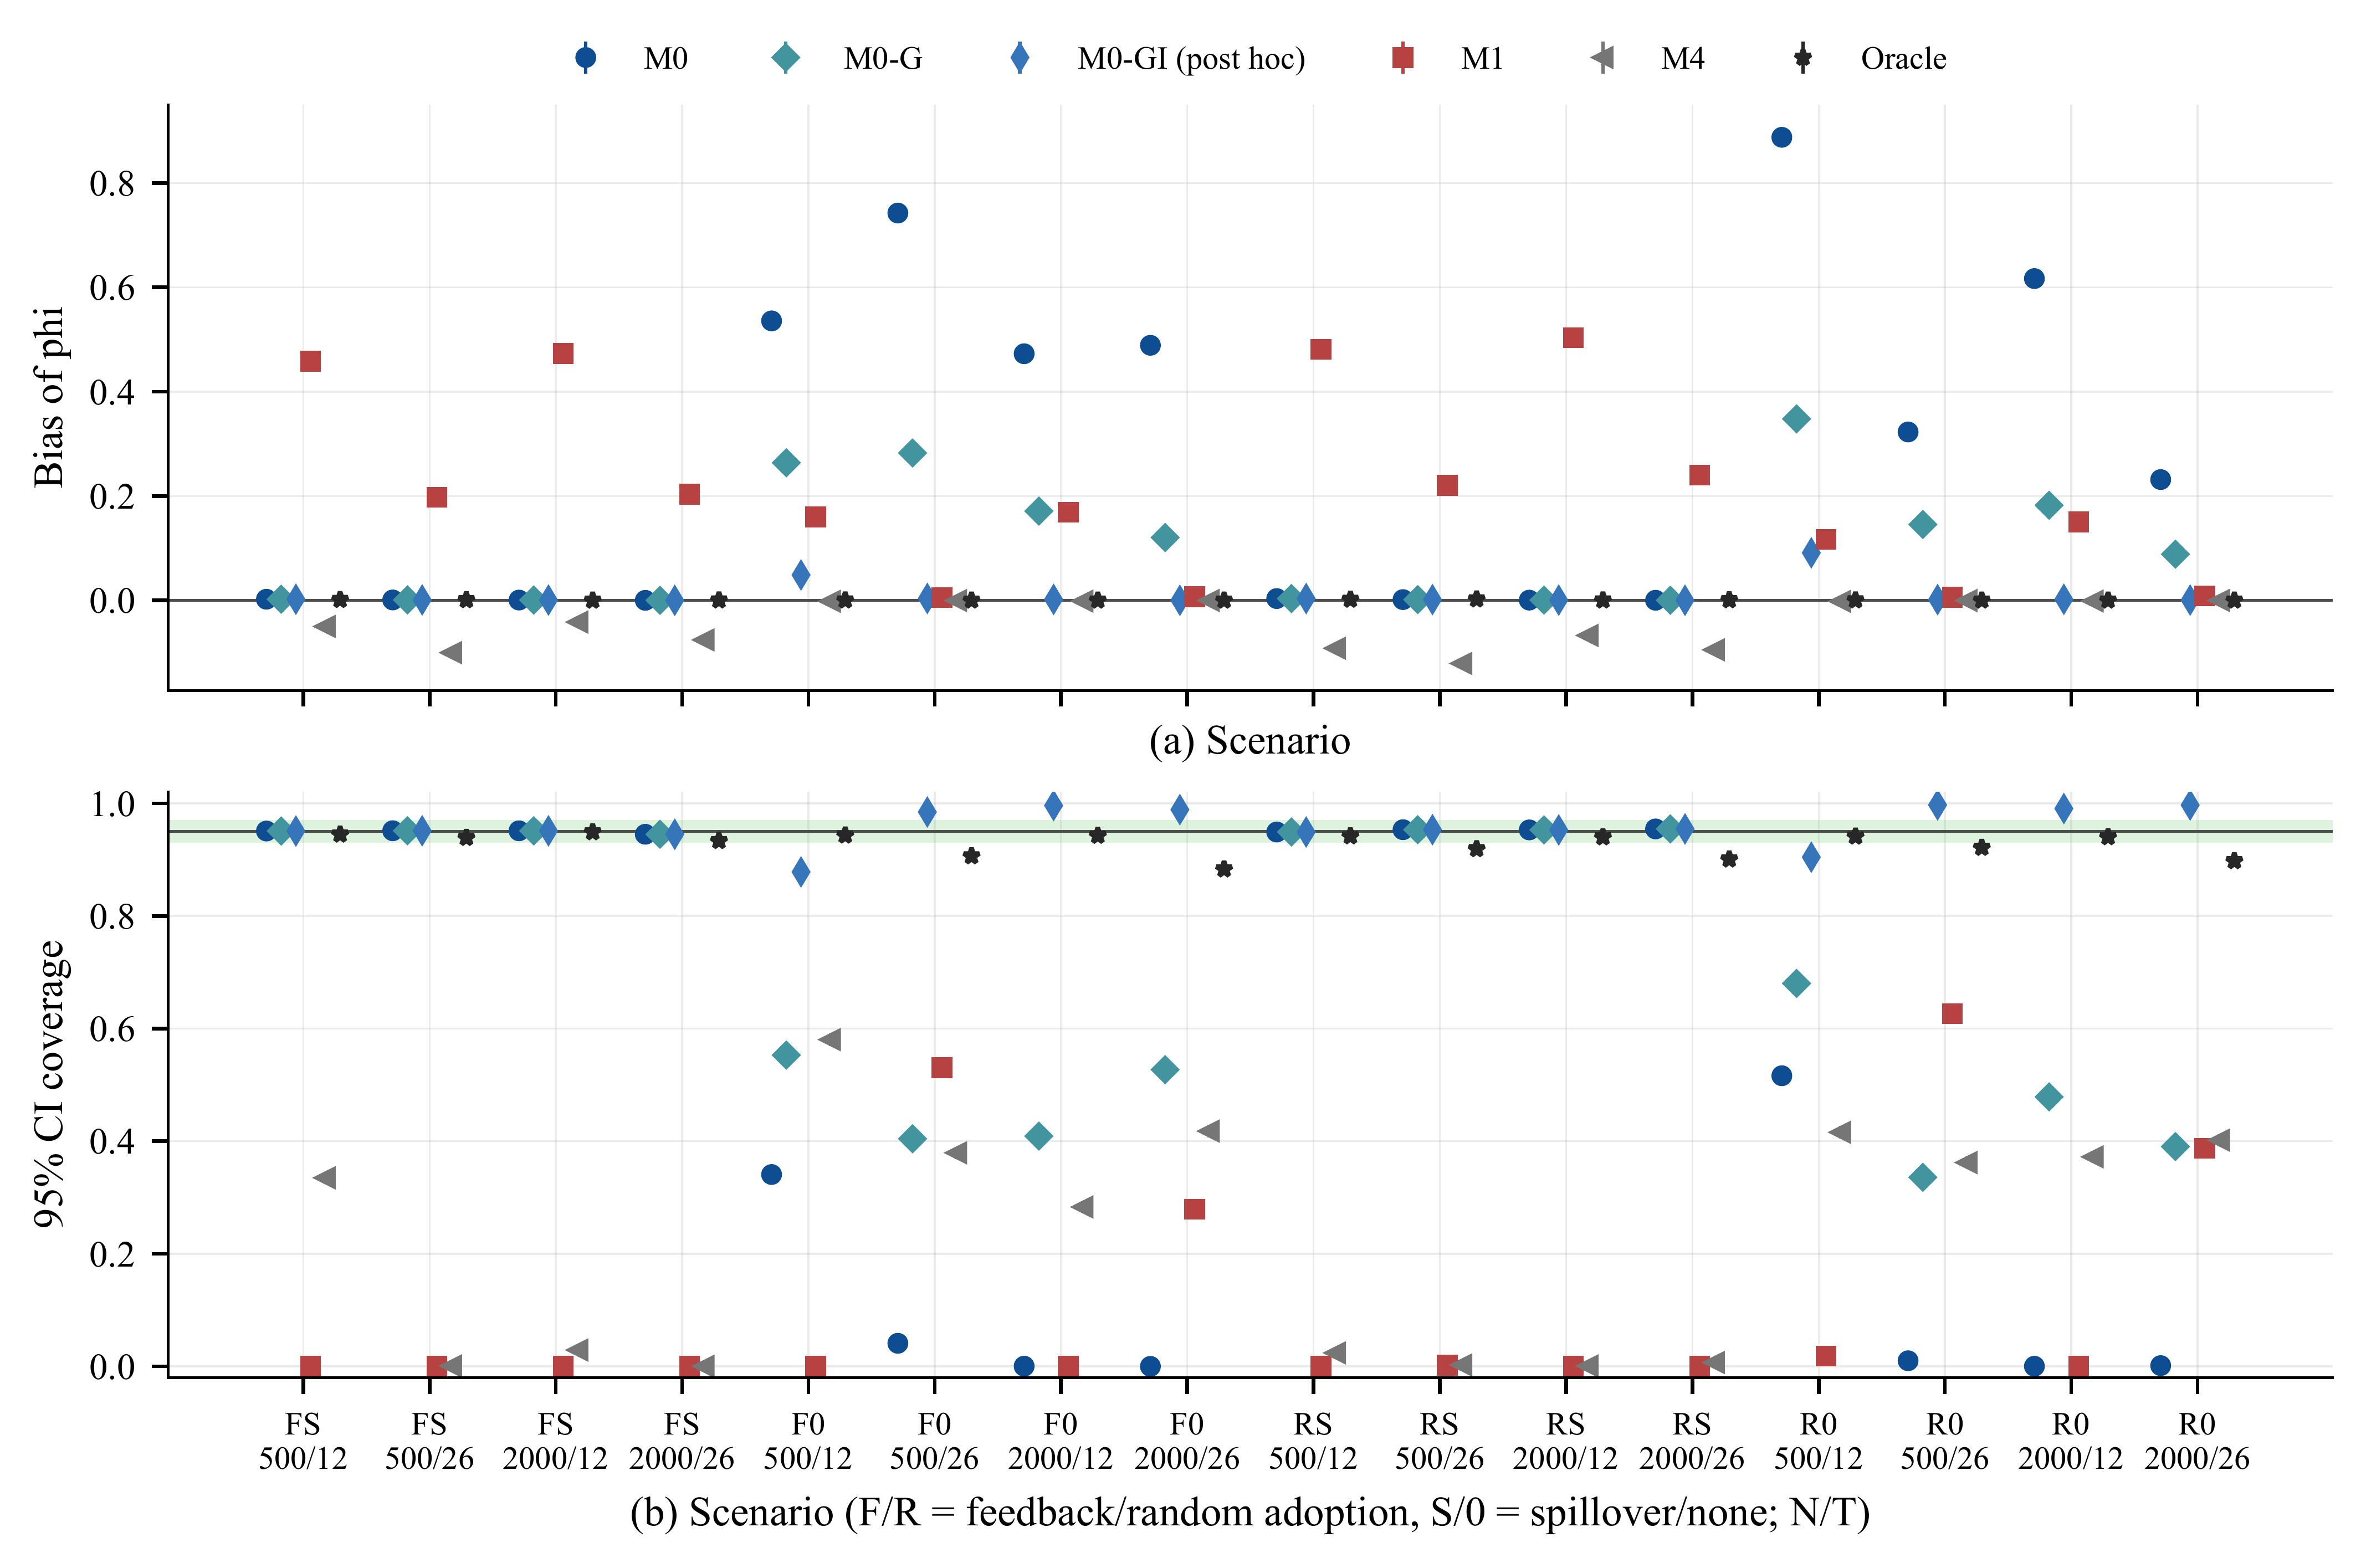
\includegraphics[width=\linewidth]{figures/fig_04_core_phi.png}
\caption{Spillover-scale parameter $\phi$, laid out as Figure~\ref{fig:core-tau}, with bias in
panel (a) and interval coverage in panel (b). The true value is 0.4 with spillover and 0 without;
coverage of M0-G and M0-GI is computed over interior selections. Error bars are $\pm2$ Monte Carlo
standard errors, and M0-GI is the post hoc variant.}
\label{fig:core-phi}
\end{figure}

\begin{figure}[!t]
\centering
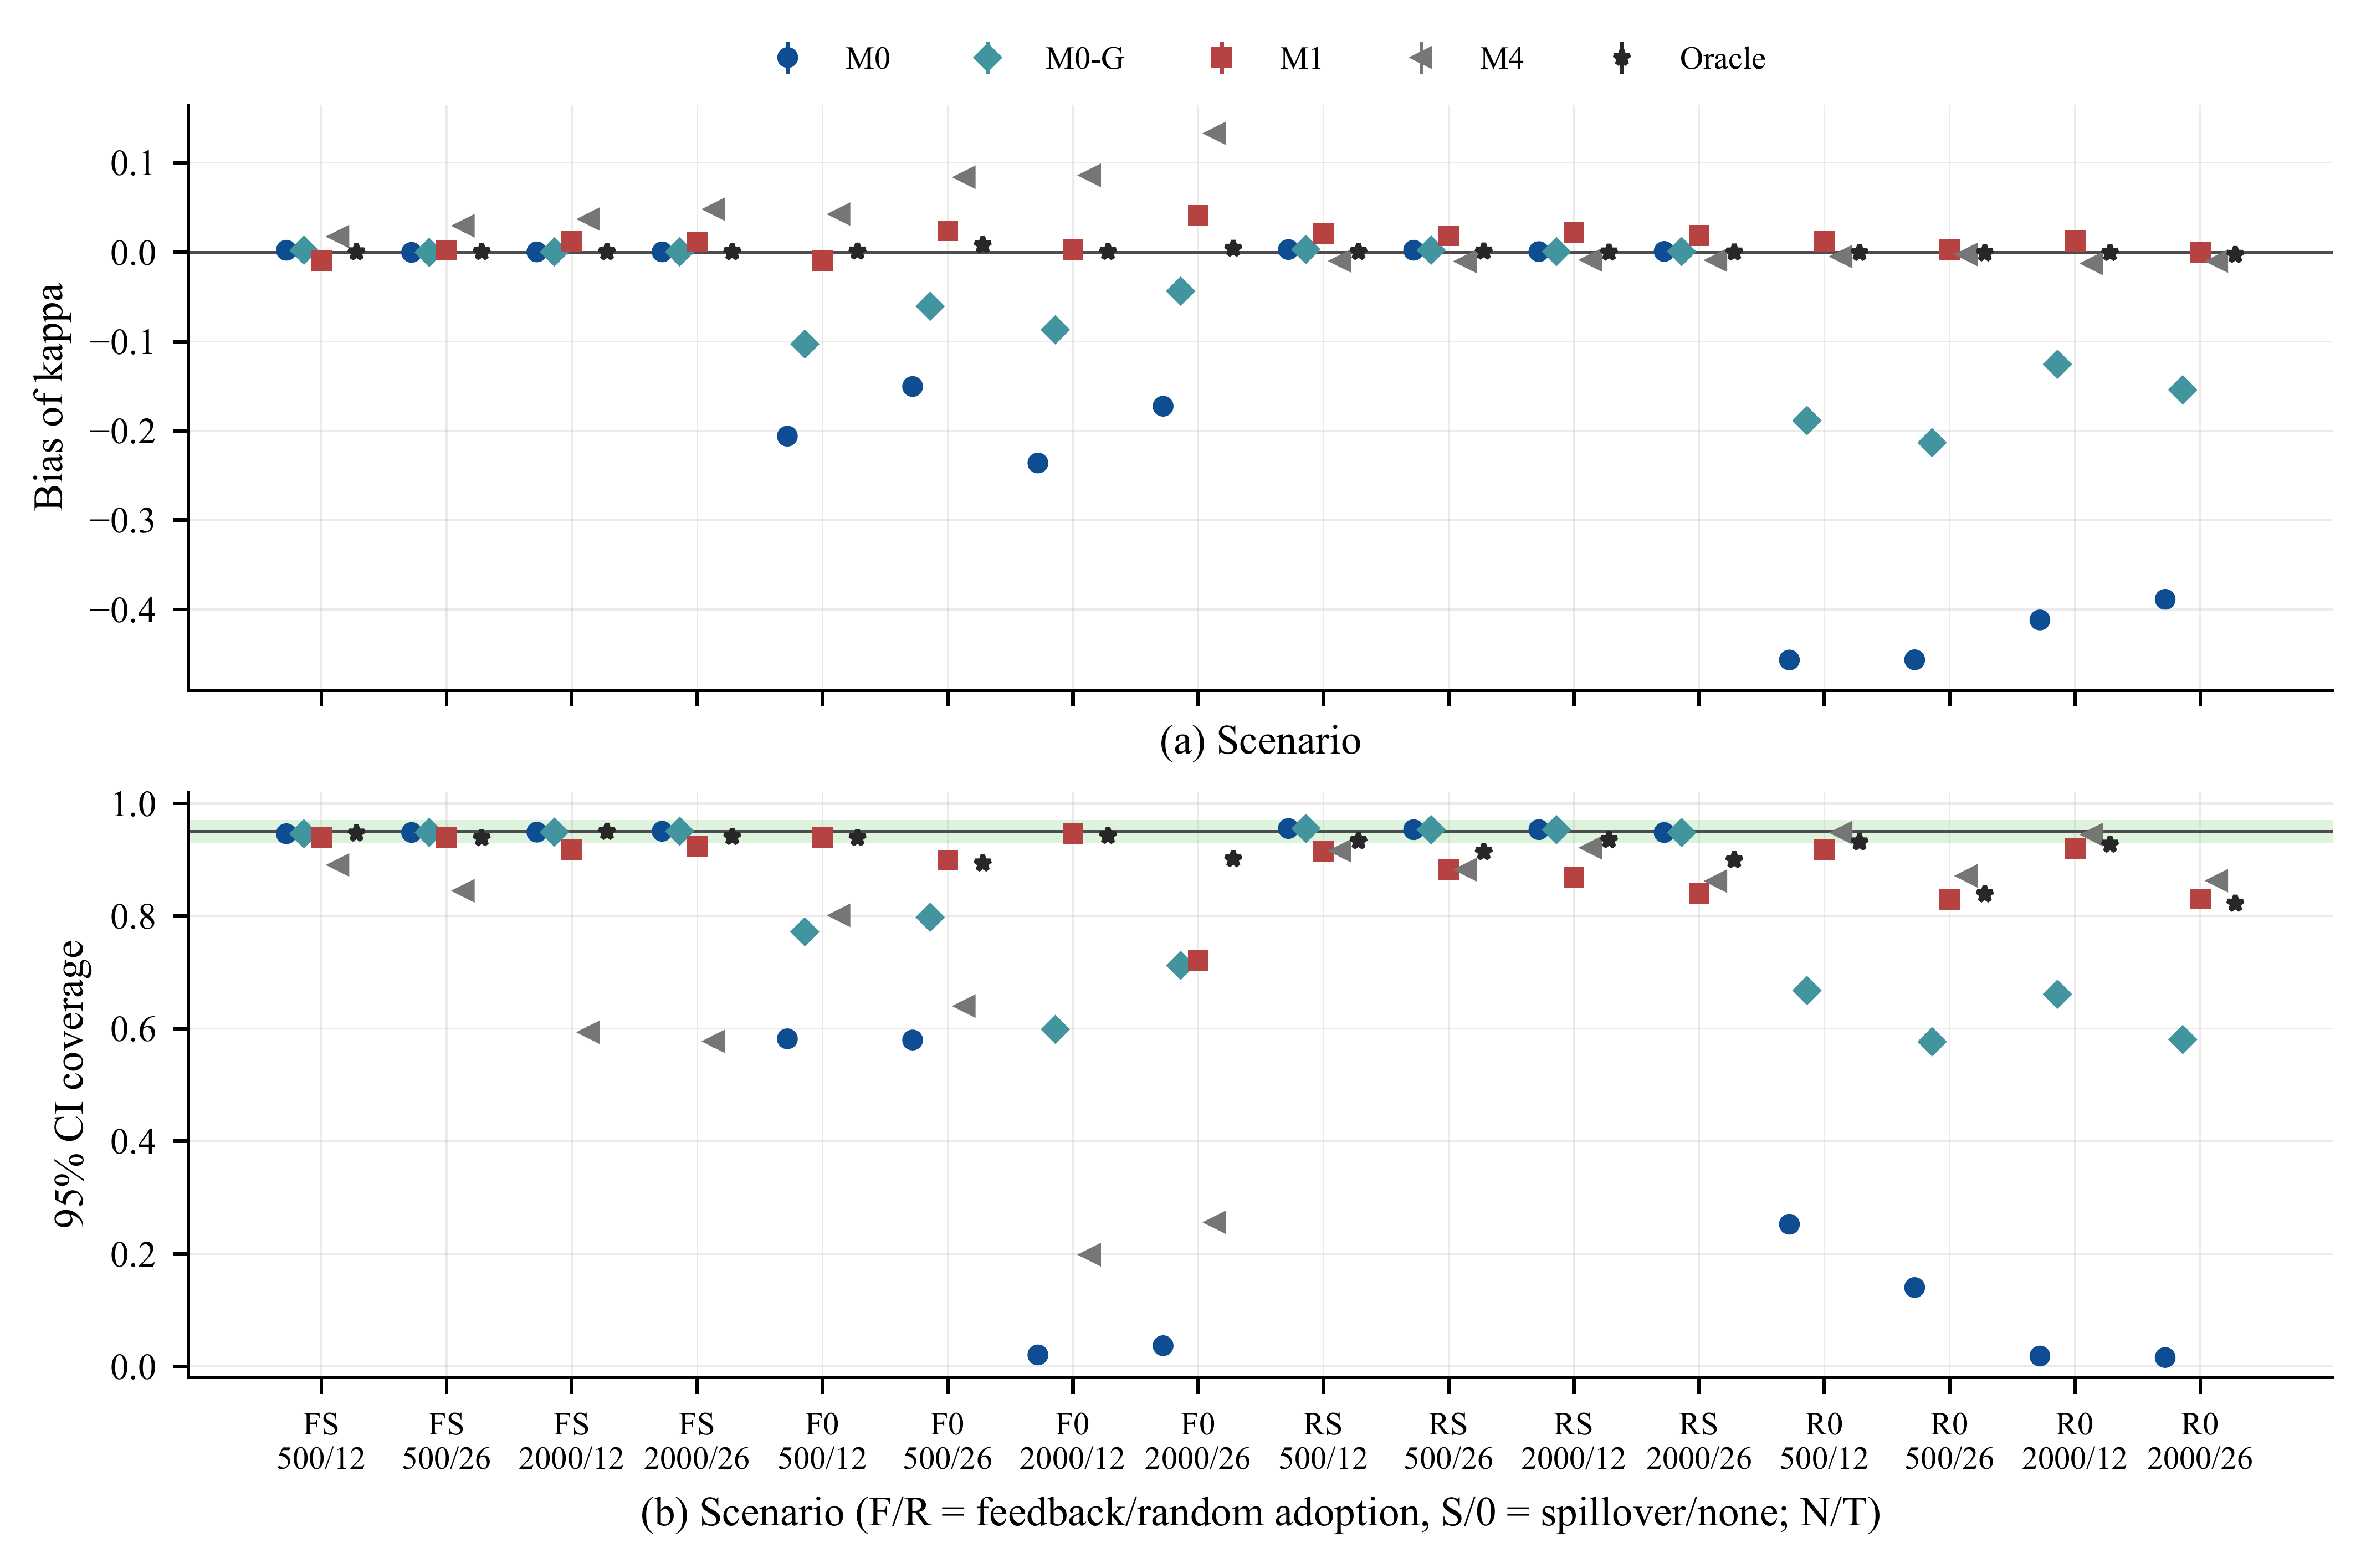
\includegraphics[width=\linewidth]{figures/fig_05_core_kappa.png}
\caption{Neighbour-policy effect $\kappa$, laid out as Figure~\ref{fig:core-tau}, with bias in
panel (a) and interval coverage in panel (b), and $\pm2$ Monte Carlo standard errors.}
\label{fig:core-kappa}
\end{figure}

\begin{figure}[!t]
\centering
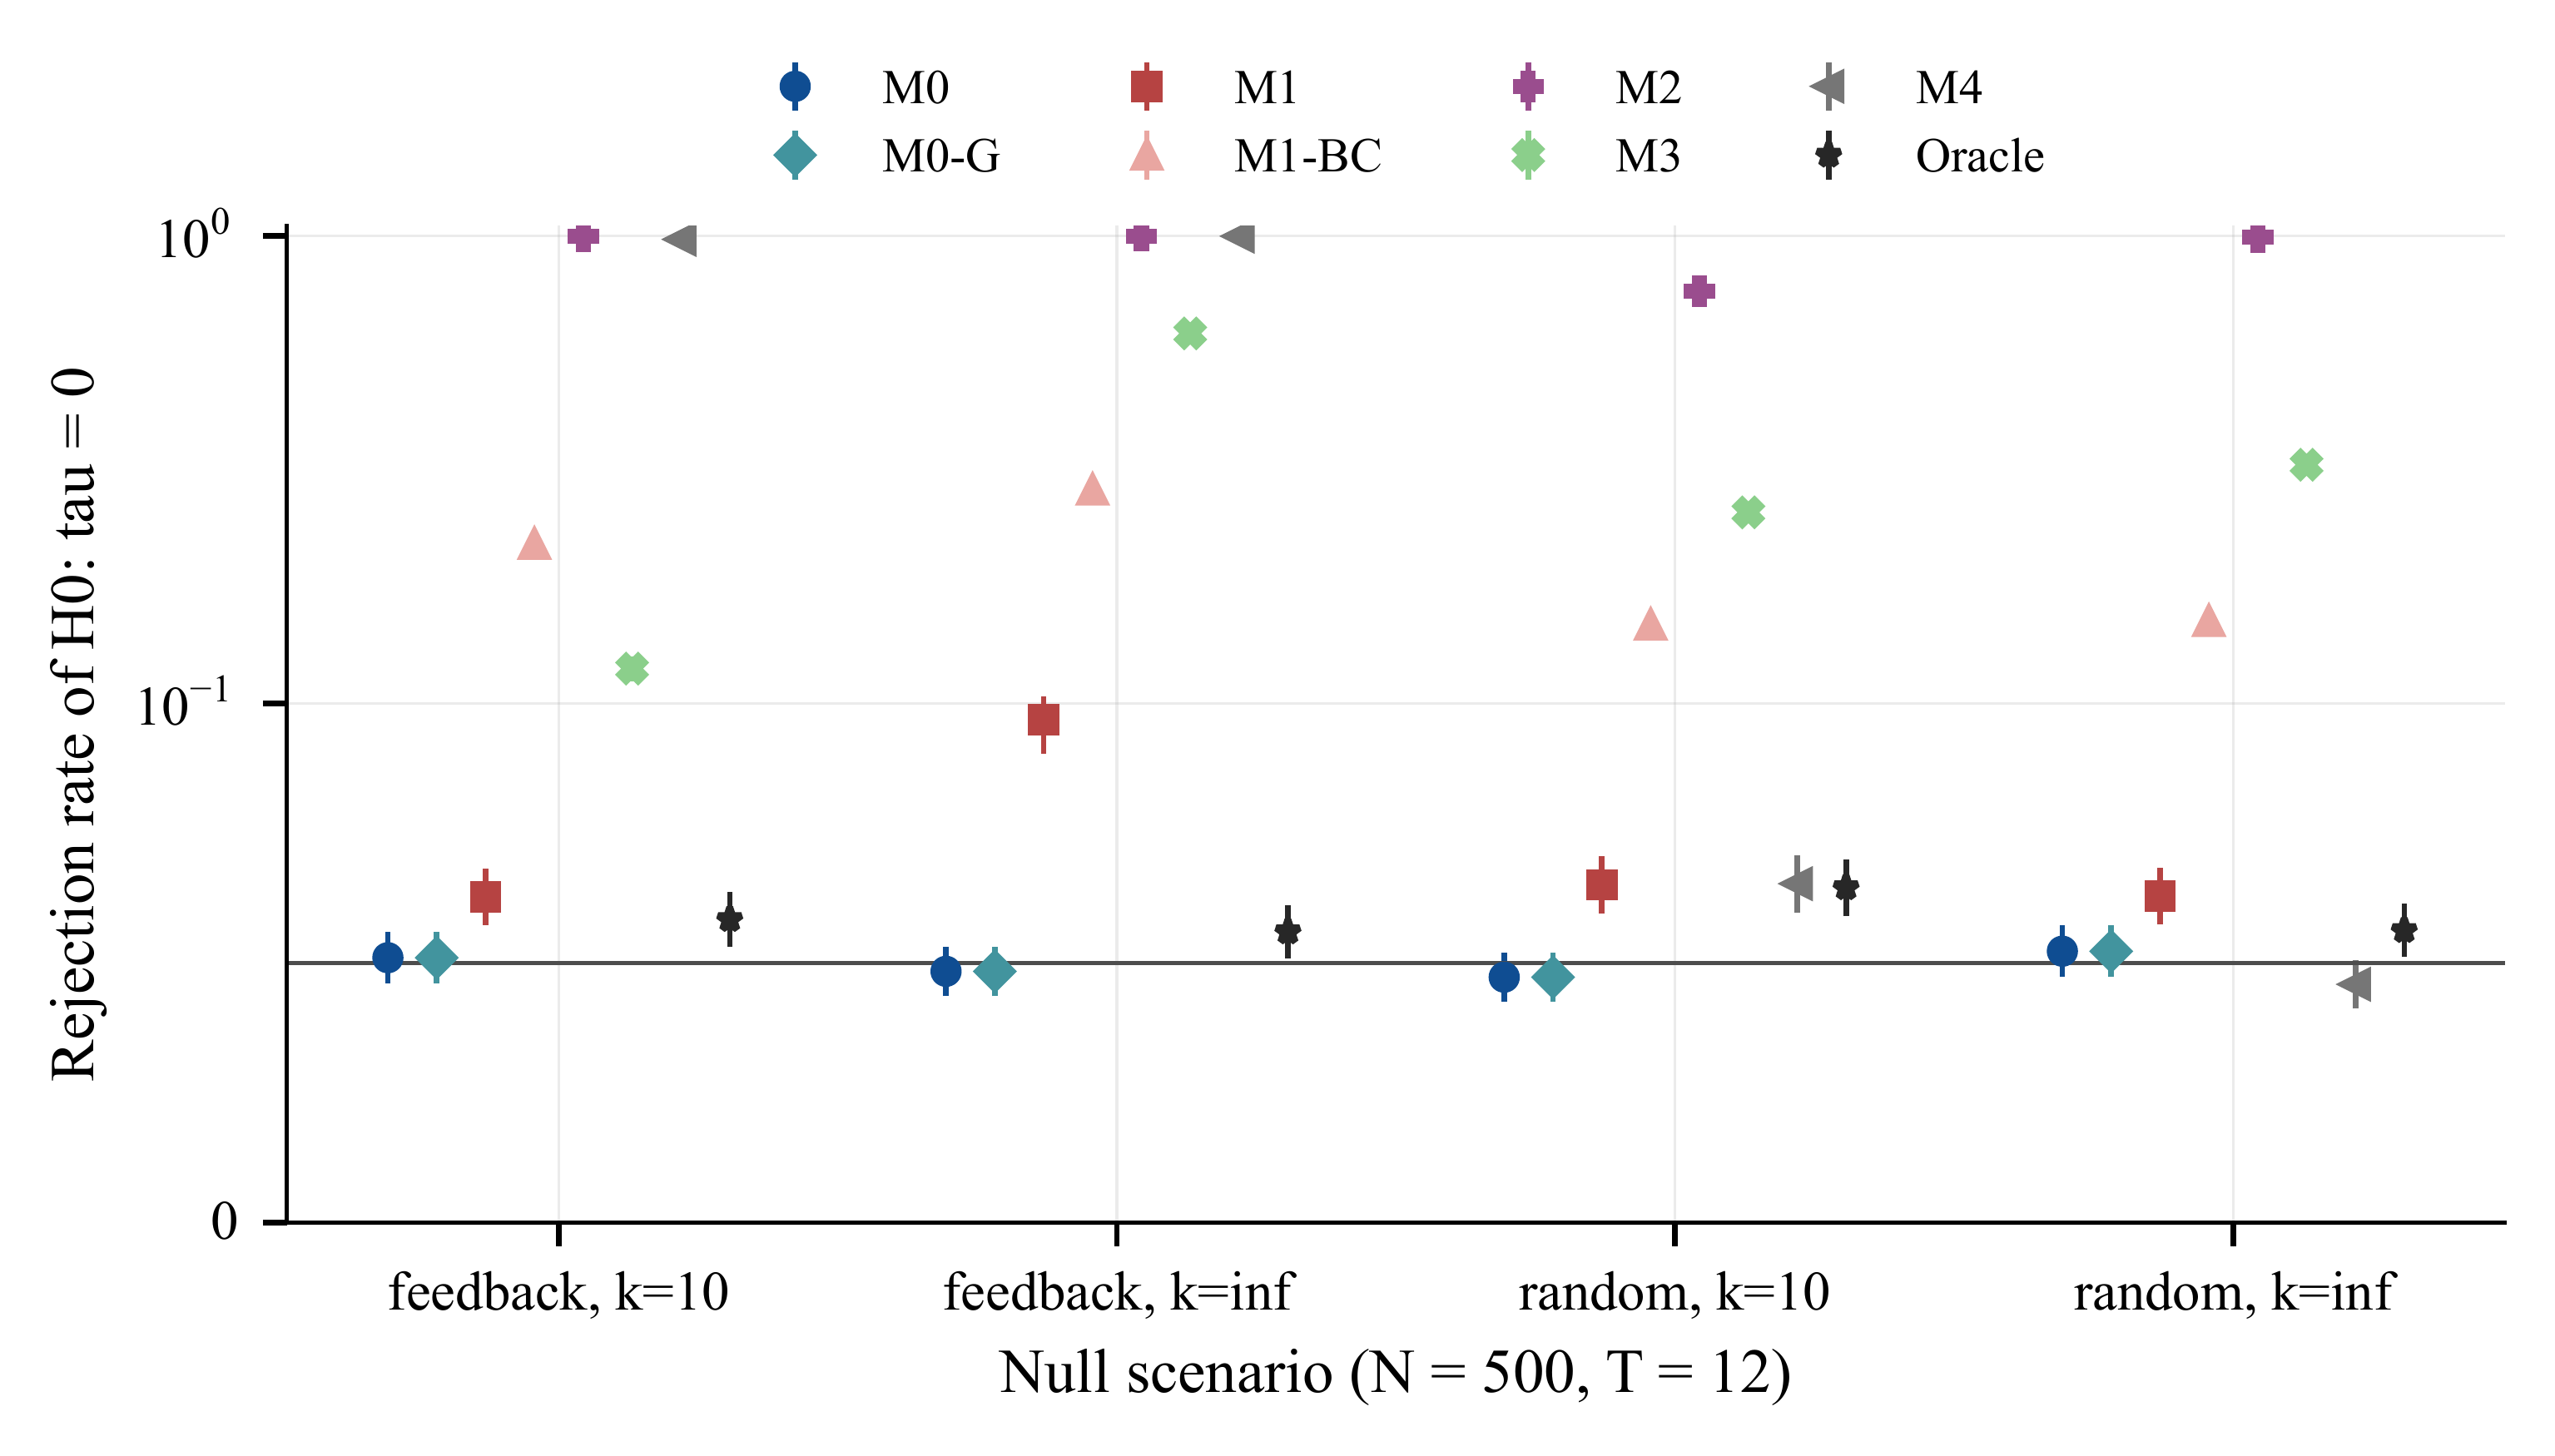
\includegraphics[width=0.93\linewidth]{figures/fig_06_null_typeI.png}
\caption{Type I error in the null block (scenarios 17--20), measured as the rejection rate of $H_0\colon\tau=0$ by
the 5\%-level $t_{G-1}$ test, by scenario and method. The horizontal line marks the nominal level, and
error bars are $\pm2$ Monte Carlo standard errors.}
\label{fig:null}
\end{figure}

\begin{figure}[!t]
\centering
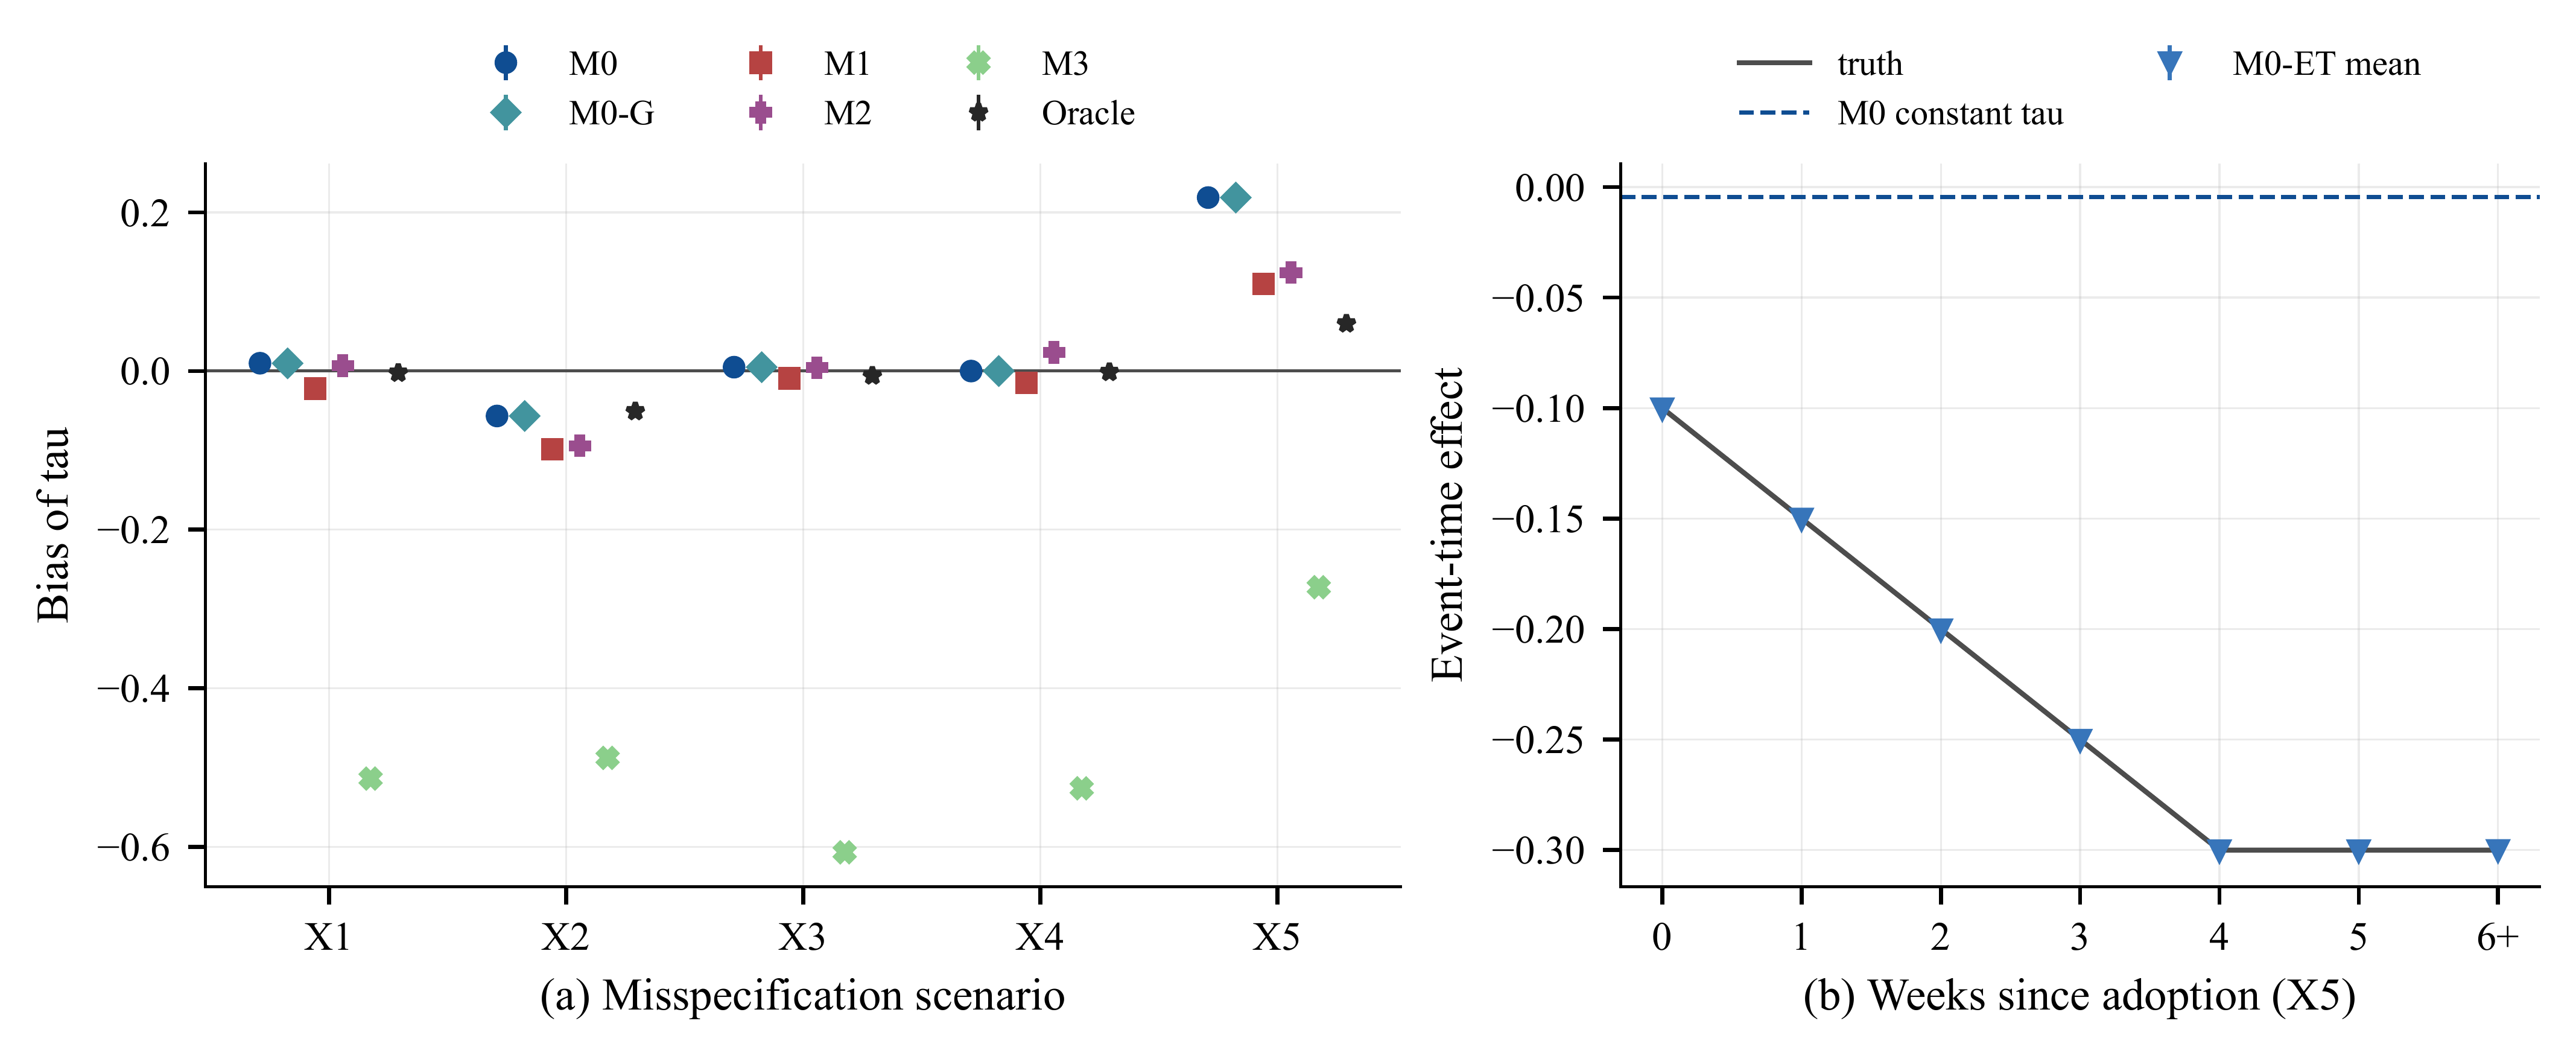
\includegraphics[width=0.93\linewidth]{figures/fig_07_misspec.png}
\caption{Misspecification block (scenarios X1--X5). (a) Bias of $\hat\tau$ by method, with $\pm2$
Monte Carlo standard errors. (b) Scenario X5, with effects growing with time since adoption, shows mean M0-ET
event-time estimates ($\pm2$ Monte Carlo standard errors) against the generating effects and the
constant-effect M0 estimate.}
\label{fig:misspec}
\end{figure}

\begin{table}[!t]
\centering
\caption{Full performance measures for M0 ($\tau$), all scenarios: bias (mean over replications), empirical and model standard errors, RMSE and coverage of nominal 95\% confidence intervals, with Monte Carlo standard errors.}
\label{tab:sim-m0-full}
\footnotesize
\setlength{\tabcolsep}{3.5pt}
\begin{adjustbox}{max width=\linewidth}
\begin{tabular}{lrrrrrrr}
\toprule
scenario & bias (MCSE) & empSE (MCSE) & modSE & rel.\ err.\ SE (MCSE) & RMSE (MCSE) & cov.\ (MCSE) & conv. \\
\midrule
1 $N=500$, $T=12$, FB, spill & -0.002 (0.001) & 0.068 (0.001) & 0.067 & -0.012 (0.008) & 0.068 (0.001) & 94.8 (0.2) & 100.0 \\
2 $N=500$, $T=26$, FB, spill & -0.000 (0.001) & 0.055 (0.000) & 0.055 & -0.015 (0.008) & 0.055 (0.000) & 94.5 (0.3) & 100.0 \\
3 $N=2000$, $T=12$, FB, spill & 0.000 (0.000) & 0.041 (0.000) & 0.040 & -0.011 (0.008) & 0.041 (0.000) & 95.0 (0.2) & 100.0 \\
4 $N=2000$, $T=26$, FB, spill & -0.000 (0.000) & 0.037 (0.000) & 0.037 & -0.007 (0.008) & 0.037 (0.000) & 94.9 (0.2) & 100.0 \\
5 $N=500$, $T=12$, FB, no spill & 0.170 (0.001) & 0.075 (0.001) & 0.455 & 5.089 (1.65e+04) & 0.186 (0.001) & 38.8 (0.6) & 97.8 \\
6 $N=500$, $T=26$, FB, no spill & 0.132 (0.001) & 0.055 (0.000) & 0.056 & 0.019 (0.008) & 0.143 (0.001) & 36.0 (0.5) & 99.3 \\
7 $N=2000$, $T=12$, FB, no spill & 0.198 (0.000) & 0.044 (0.000) & 0.043 & -0.019 (0.008) & 0.203 (0.000) & 0.6 (0.1) & 100.0 \\
8 $N=2000$, $T=26$, FB, no spill & 0.154 (0.000) & 0.035 (0.000) & 0.036 & 0.029 (0.008) & 0.158 (0.000) & 0.9 (0.1) & 100.0 \\
9 $N=500$, $T=12$, RD, spill & -0.001 (0.001) & 0.082 (0.001) & 0.081 & -0.006 (0.008) & 0.082 (0.001) & 95.4 (0.2) & 100.0 \\
10 $N=500$, $T=26$, RD, spill & 0.001 (0.001) & 0.070 (0.001) & 0.069 & -0.012 (0.008) & 0.070 (0.001) & 95.2 (0.2) & 100.0 \\
11 $N=2000$, $T=12$, RD, spill & -0.001 (0.001) & 0.063 (0.001) & 0.063 & -0.009 (0.008) & 0.063 (0.001) & 95.3 (0.2) & 100.0 \\
12 $N=2000$, $T=26$, RD, spill & 0.000 (0.001) & 0.054 (0.000) & 0.054 & -0.016 (0.008) & 0.054 (0.000) & 94.6 (0.3) & 100.0 \\
13 $N=500$, $T=12$, RD, no spill & 0.469 (0.002) & 0.182 (0.001) & 0.176 & -0.035 (0.072) & 0.504 (0.002) & 12.1 (0.4) & 92.9 \\
14 $N=500$, $T=26$, RD, no spill & 0.431 (0.002) & 0.148 (0.001) & 0.127 & -0.139 (0.008) & 0.455 (0.002) & 4.6 (0.2) & 100.0 \\
15 $N=2000$, $T=12$, RD, no spill & 0.405 (0.001) & 0.123 (0.001) & 0.103 & -0.162 (0.007) & 0.424 (0.001) & 0.7 (0.1) & 100.0 \\
16 $N=2000$, $T=26$, RD, no spill & 0.363 (0.001) & 0.104 (0.001) & 0.089 & -0.145 (0.007) & 0.377 (0.001) & 1.0 (0.1) & 100.0 \\
17 $N=500$, $T=12$, FB, $k=10$ & -0.001 (0.001) & 0.055 (0.000) & 0.055 & -0.012 (0.008) & 0.055 (0.000) & 94.9 (0.2) & 100.0 \\
18 $N=500$, $T=12$, FB, $k=\infty$ & -0.000 (0.000) & 0.029 (0.000) & 0.029 & 0.001 (0.008) & 0.029 (0.000) & 95.2 (0.2) & 100.0 \\
19 $N=500$, $T=12$, RD, $k=10$ & 0.001 (0.001) & 0.077 (0.001) & 0.076 & -0.019 (0.008) & 0.077 (0.001) & 95.3 (0.2) & 100.0 \\
20 $N=500$, $T=12$, RD, $k=\infty$ & 0.001 (0.000) & 0.039 (0.000) & 0.038 & -0.033 (0.008) & 0.039 (0.000) & 94.8 (0.2) & 100.0 \\
21 X1: wrong generation interval & 0.010 (0.000) & 0.036 (0.000) & 0.036 & 0.015 (0.008) & 0.037 (0.000) & 94.6 (0.3) & 100.0 \\
22 X2: reporting drops after adoption & -0.057 (0.000) & 0.032 (0.000) & 0.032 & 0.018 (0.008) & 0.065 (0.000) & 59.4 (0.5) & 100.0 \\
23 X3: heterogeneous effects & 0.005 (0.000) & 0.038 (0.000) & 0.037 & -0.018 (0.008) & 0.038 (0.000) & 94.0 (0.3) & 100.0 \\
24 X4: susceptible depletion & -0.000 (0.000) & 0.037 (0.000) & 0.037 & -0.007 (0.008) & 0.037 (0.000) & 95.2 (0.2) & 100.0 \\
25 X5: dynamic effects & 0.219 (0.000) & 0.038 (0.000) & 0.039 & 0.035 (0.008) & 0.222 (0.000) & 0.0 (0.0) & 100.0 \\
\bottomrule
\end{tabular}
\end{adjustbox}
\par\smallskip\parbox{\linewidth}{\scriptsize Primary estimator M0, $\tau$: Monte Carlo performance measures with Monte Carlo standard errors (Morris, White and Crowther, 2019). empSE = sd of $\hat\tau$ (ddof 1); modSE = mean cluster-robust SE; rel.\ err.\ SE = modSE/empSE$-1$; cov.\ (\%) of 95\% $t_{G-1}$ intervals; conv.\ = share (\%) of replications in which the solver converged. In Scenario~5 ($\phi_0=0$, no spillover), arithmetic mean SE (0.455, rel.\ err.\ 5.089, MCSE $1.65\times 10^4$) is dominated by $<0.6\%$ extreme near-boundary Jacobian draws (e.g.\ SE $>2900$ at $\hat\phi\approx 0.09$); over $R=400$ diagnostic draws, median SE is 0.074 (IQR 0.015, $+6.4\%$ vs.\ empSD). R = 8000 per scenario.}
\end{table}


\begin{table}[!t]
\centering
\caption{Bias (mean of estimate minus true value) and coverage of nominal 95\% confidence intervals for the spillover parameters $\kappa$ and $\phi$ (core scenarios).}
\label{tab:sim-core-spill}
\footnotesize
\setlength{\tabcolsep}{3.5pt}
\begin{adjustbox}{max width=\linewidth}
\begin{tabular}{ccccrrrrrrrrrrrrrrrrrrrr}
\toprule
$N$ & $T$ & adopt & spill & \multicolumn{4}{c}{M0} & \multicolumn{4}{c}{M0-G} & \multicolumn{4}{c}{M1} & \multicolumn{4}{c}{M4} & \multicolumn{4}{c}{Oracle} \\
\cmidrule(lr){5-8}\cmidrule(lr){9-12}\cmidrule(lr){13-16}\cmidrule(lr){17-20}\cmidrule(lr){21-24}
 & & & & \multicolumn{2}{c}{$\kappa$} & \multicolumn{2}{c}{$\phi$} & \multicolumn{2}{c}{$\kappa$} & \multicolumn{2}{c}{$\phi$} & \multicolumn{2}{c}{$\kappa$} & \multicolumn{2}{c}{$\phi$} & \multicolumn{2}{c}{$\kappa$} & \multicolumn{2}{c}{$\phi$} & \multicolumn{2}{c}{$\kappa$} & \multicolumn{2}{c}{$\phi$} \\
 & & & & bias & cov & bias & cov & bias & cov & bias & cov & bias & cov & bias & cov & bias & cov & bias & cov & bias & cov & bias & cov \\
\midrule
500 & 12 & FB & yes & 0.002 & 94.6 & 0.002 & 95.1 & 0.002 & 94.6 & 0.002 & 95.1 & -0.009 & 93.9 & 0.458 & 0.0 & 0.017 & 89.1 & -0.050 & 33.5 & 0.000 & 94.7 & 0.001 & 94.5 \\
500 & 26 & FB & yes & -0.000 & 94.8 & 0.001 & 95.1 & -0.000 & 94.8 & 0.001 & 95.1 & 0.002 & 94.0 & 0.197 & 0.0 & 0.029 & 84.5 & -0.100 & 0.1 & 0.000 & 93.8 & 0.001 & 93.9 \\
2000 & 12 & FB & yes & 0.000 & 94.9 & 0.001 & 95.1 & 0.000 & 94.9 & 0.001 & 95.1 & 0.012 & 91.8 & 0.473 & 0.0 & 0.037 & 59.3 & -0.042 & 2.9 & 0.000 & 95.0 & 0.000 & 94.9 \\
2000 & 26 & FB & yes & 0.000 & 95.0 & 0.000 & 94.5 & 0.000 & 95.0 & 0.000 & 94.5 & 0.011 & 92.3 & 0.204 & 0.0 & 0.048 & 57.7 & -0.076 & 0.0 & 0.000 & 94.1 & 0.000 & 93.3 \\
500 & 12 & FB & no & -0.206 & 58.2 & 0.536 & 34.1 & -0.103 & 77.2 & 0.264 & 55.3 & -0.010 & 94.0 & 0.160 & 0.0 & 0.043 & 80.1 & -0.002 & 58.0 & 0.001 & 93.9 & 0.000 & 94.3 \\
500 & 26 & FB & no & -0.150 & 58.0 & 0.742 & 4.1 & -0.061 & 79.8 & 0.283 & 40.4 & 0.024 & 89.9 & 0.006 & 53.0 & 0.084 & 64.0 & -0.000 & 37.9 & 0.008 & 89.4 & 0.000 & 90.6 \\
2000 & 12 & FB & no & -0.236 & 2.0 & 0.473 & 0.0 & -0.087 & 59.9 & 0.171 & 40.9 & 0.003 & 94.6 & 0.169 & 0.0 & 0.086 & 19.8 & -0.001 & 28.3 & 0.000 & 94.3 & 0.000 & 94.3 \\
2000 & 26 & FB & no & -0.173 & 3.7 & 0.489 & 0.0 & -0.044 & 71.2 & 0.120 & 52.7 & 0.041 & 72.1 & 0.007 & 27.9 & 0.133 & 25.6 & -0.000 & 41.8 & 0.004 & 90.1 & 0.000 & 88.3 \\
500 & 12 & RD & yes & 0.003 & 95.5 & 0.004 & 94.9 & 0.003 & 95.5 & 0.004 & 94.9 & 0.020 & 91.4 & 0.481 & 0.0 & -0.010 & 91.6 & -0.092 & 2.4 & 0.000 & 93.3 & 0.002 & 94.2 \\
500 & 26 & RD & yes & 0.002 & 95.3 & 0.002 & 95.3 & 0.002 & 95.3 & 0.002 & 95.3 & 0.018 & 88.2 & 0.221 & 0.2 & -0.010 & 88.2 & -0.121 & 0.2 & 0.001 & 91.4 & 0.002 & 91.9 \\
2000 & 12 & RD & yes & 0.001 & 95.3 & 0.001 & 95.3 & 0.001 & 95.3 & 0.001 & 95.3 & 0.022 & 86.8 & 0.503 & 0.0 & -0.009 & 92.1 & -0.067 & 0.1 & -0.000 & 93.5 & 0.000 & 94.0 \\
2000 & 26 & RD & yes & 0.001 & 94.8 & 0.000 & 95.5 & 0.001 & 94.8 & 0.000 & 95.5 & 0.019 & 84.0 & 0.240 & 0.0 & -0.009 & 86.2 & -0.095 & 0.7 & -0.000 & 90.0 & 0.001 & 90.1 \\
500 & 12 & RD & no & -0.457 & 25.2 & 0.888 & 51.6 & -0.189 & 66.8 & 0.348 & 68.0 & 0.012 & 91.8 & 0.117 & 1.8 & -0.005 & 94.8 & -0.002 & 41.6 & -0.001 & 93.1 & 0.001 & 94.1 \\
500 & 26 & RD & no & -0.456 & 14.0 & 0.323 & 1.0 & -0.213 & 57.7 & 0.146 & 33.6 & 0.003 & 82.9 & 0.006 & 62.7 & -0.003 & 87.1 & -0.000 & 36.2 & -0.001 & 83.9 & 0.000 & 92.1 \\
2000 & 12 & RD & no & -0.412 & 1.8 & 0.617 & 0.0 & -0.126 & 66.1 & 0.182 & 47.9 & 0.012 & 92.0 & 0.151 & 0.0 & -0.013 & 94.5 & -0.001 & 37.2 & -0.001 & 92.7 & 0.000 & 94.0 \\
2000 & 26 & RD & no & -0.389 & 1.6 & 0.232 & 0.1 & -0.154 & 58.1 & 0.089 & 39.0 & 0.000 & 83.0 & 0.009 & 38.7 & -0.010 & 86.3 & -0.000 & 40.2 & -0.003 & 82.2 & 0.000 & 89.8 \\
\bottomrule
\end{tabular}
\end{adjustbox}
\par\smallskip\parbox{\linewidth}{\scriptsize Spillover parameters in the core scenarios (truth $(\kappa_0,\phi_0)=(-0.1,0.4)$ with spillover, $(0,0)$ without). For M0-G, $\phi$ coverage is computed over replications whose selected solution is interior; boundary selections ($\hat\phi=0$) have no Wald interval for $\phi$ (shares in Web Table~\ref{tab:sim-roots}). R = 8000 per scenario; largest MCSE: bias 0.006, coverage 0.8 (percentage points).}
\end{table}


\begin{table}[!t]
\centering
\caption{Type I error: rejection rate of the 5\%-level $t_{G-1}$ test of $H_0\colon \tau = 0$ when the null holds.}
\label{tab:sim-null}
\footnotesize
\setlength{\tabcolsep}{3.5pt}
\begin{adjustbox}{max width=\linewidth}
\begin{tabular}{lrrrrrrrrrr}
\toprule
scenario & M0 & M0-G & M0-ET & M1 & M1-BC & M2 & M3 & M4 & Oracle & $J$ (M0-OI) \\
\midrule
FB, $k=10$ & 5.1 & 5.1 & 4.4 & 6.3 & 21.9 & 100.0 & 11.9 & 98.4 & 5.8 & 4.9 \\
FB, $k=\infty$ & 4.8 & 4.8 & 3.9 & 9.7 & 28.6 & 100.0 & 61.9 & 100.0 & 5.6 & 4.4 \\
RD, $k=10$ & 4.7 & 4.7 & 4.5 & 6.5 & 14.7 & 76.1 & 25.6 & 6.5 & 6.5 & 4.9 \\
RD, $k=\infty$ & 5.2 & 5.2 & 4.9 & 6.3 & 15.0 & 99.5 & 32.4 & 4.6 & 5.6 & 4.8 \\
\bottomrule
\end{tabular}
\end{adjustbox}
\par\smallskip\parbox{\linewidth}{\scriptsize Null block ($\tau_0=0$, $N=500$, $T=12$, spillover present): rejection rate (\%) of $H_0{:}\,\tau=0$ at nominal 5\% with $t_{G-1}$ critical values (M0-ET: first event-time bin), and rejection rate of the Hansen $J$ test of M0-OI at 5\%. $k$ = negative-binomial dispersion ($\infty$ = Poisson). R = 8000 per scenario; largest MCSE 0.5 percentage points.}
\end{table}


\begin{table}[!t]
\centering
\caption{Multiple roots and boundary solutions of the QD-GMM equations.}
\label{tab:sim-roots}
\footnotesize
\setlength{\tabcolsep}{3.5pt}
\begin{adjustbox}{max width=\linewidth}
\begin{tabular}{lrrrrrrr}
\toprule
scenario & $\phi_0$ & conv.\ M0 & conv.\ M0-G & $>1$ root & no interior root & boundary & M0-G $\neq$ M0 \\
\midrule
1 $N=500$, $T=12$, FB, spill & 0.4 & 100.0 & 100.0 & 0.0 & 0.0 & 0.0 & 0.0 \\
2 $N=500$, $T=26$, FB, spill & 0.4 & 100.0 & 100.0 & 0.0 & 0.0 & 0.0 & 0.0 \\
3 $N=2000$, $T=12$, FB, spill & 0.4 & 100.0 & 100.0 & 0.0 & 0.0 & 0.0 & 0.0 \\
4 $N=2000$, $T=26$, FB, spill & 0.4 & 100.0 & 100.0 & 0.0 & 0.0 & 0.0 & 0.0 \\
5 $N=500$, $T=12$, FB, no spill & 0.0 & 97.8 & 100.0 & 48.3 & 2.3 & 28.6 & 49.7 \\
6 $N=500$, $T=26$, FB, no spill & 0.0 & 99.3 & 100.0 & 51.7 & 0.5 & 33.6 & 59.1 \\
7 $N=2000$, $T=12$, FB, no spill & 0.0 & 100.0 & 100.0 & 50.0 & 0.0 & 36.6 & 62.5 \\
8 $N=2000$, $T=26$, FB, no spill & 0.0 & 100.0 & 100.0 & 51.0 & 0.0 & 44.8 & 74.2 \\
9 $N=500$, $T=12$, RD, spill & 0.4 & 100.0 & 100.0 & 0.0 & 0.0 & 0.0 & 0.0 \\
10 $N=500$, $T=26$, RD, spill & 0.4 & 100.0 & 100.0 & 0.0 & 0.0 & 0.0 & 0.0 \\
11 $N=2000$, $T=12$, RD, spill & 0.4 & 100.0 & 100.0 & 0.0 & 0.0 & 0.0 & 0.0 \\
12 $N=2000$, $T=26$, RD, spill & 0.4 & 100.0 & 100.0 & 0.0 & 0.0 & 0.0 & 0.0 \\
13 $N=500$, $T=12$, RD, no spill & 0.0 & 92.9 & 100.0 & 47.2 & 5.8 & 33.6 & 55.3 \\
14 $N=500$, $T=26$, RD, no spill & 0.0 & 100.0 & 100.0 & 50.1 & 0.1 & 30.2 & 53.2 \\
15 $N=2000$, $T=12$, RD, no spill & 0.0 & 100.0 & 100.0 & 50.1 & 0.0 & 40.4 & 69.0 \\
16 $N=2000$, $T=26$, RD, no spill & 0.0 & 100.0 & 100.0 & 50.2 & 0.0 & 34.8 & 60.4 \\
17 $N=500$, $T=12$, FB, $k=10$ & 0.4 & 100.0 & 100.0 & 0.0 & 0.0 & 0.0 & 0.0 \\
18 $N=500$, $T=12$, FB, $k=\infty$ & 0.4 & 100.0 & 100.0 & 0.0 & 0.0 & 0.0 & 0.0 \\
19 $N=500$, $T=12$, RD, $k=10$ & 0.4 & 100.0 & 100.0 & 0.0 & 0.0 & 0.0 & 0.0 \\
20 $N=500$, $T=12$, RD, $k=\infty$ & 0.4 & 100.0 & 100.0 & 0.0 & 0.0 & 0.0 & 0.0 \\
21 X1: wrong generation interval & 0.4 & 100.0 & 100.0 & 0.0 & 0.0 & 0.1 & 0.1 \\
22 X2: reporting drops after adoption & 0.4 & 100.0 & 100.0 & 0.0 & 0.0 & 0.0 & 0.0 \\
23 X3: heterogeneous effects & 0.4 & 100.0 & 100.0 & 0.0 & 0.0 & 0.0 & 0.0 \\
24 X4: susceptible depletion & 0.4 & 100.0 & 100.0 & 0.0 & 0.0 & 0.0 & 0.0 \\
25 X5: dynamic effects & 0.4 & 100.0 & 100.0 & 0.0 & 0.0 & 0.0 & 0.0 \\
\bottomrule
\end{tabular}
\end{adjustbox}
\par\smallskip\parbox{\linewidth}{\scriptsize Root diagnostics of the profiled QD-GMM equations over the grid $\phi\in[0,3]$ (M0-G): share (\%) of replications with more than one interior root, with no interior root, in which the minimum-$Q$ selection is the boundary $\phi=0$, and in which M0-G differs from M0 (local root from the pre-specified start). R = 8000.}
\end{table}


\begin{table}[!t]
\centering
\caption{Robustness of M0 under misspecification: bias (mean over replications) and coverage of nominal 95\% confidence intervals.}
\label{tab:sim-misspec}
\footnotesize
\setlength{\tabcolsep}{3.5pt}
\begin{adjustbox}{max width=\linewidth}
\begin{tabular}{lrrrrrrrrr}
\toprule
scenario & \multicolumn{2}{c}{$\tau$} & \multicolumn{2}{c}{$\kappa$} & \multicolumn{2}{c}{$\phi$} & $J$ rej. & M1 $\tau$ bias & M2 $\tau$ bias \\
\cmidrule(lr){2-3}\cmidrule(lr){4-5}\cmidrule(lr){6-7}
 & bias & cov & bias & cov & bias & cov & & & \\
\midrule
X1: wrong generation interval & 0.010 & 94.6 & -0.050 & 80.2 & 0.516 & 0.0 & 100.0 & -0.022 & 0.007 \\
X2: reporting drops after adoption & -0.057 & 59.4 & -0.294 & 0.0 & 0.424 & 0.0 & 100.0 & -0.099 & -0.094 \\
X3: heterogeneous effects & 0.005 & 94.0 & 0.000 & 94.6 & 0.000 & 95.6 & 4.4 & -0.009 & 0.004 \\
X4: susceptible depletion & -0.000 & 95.2 & -0.000 & 94.9 & -0.002 & 94.6 & 4.6 & -0.015 & 0.024 \\
X5: dynamic effects & 0.219 & 0.0 & 0.014 & 94.6 & 0.000 & 95.0 & 4.7 & 0.110 & 0.124 \\
\midrule
\multicolumn{10}{l}{X3, M0 $\tau$ vs switcher mean of $\tau_i$: bias 0.005, coverage 94.0\%} \\
\multicolumn{10}{l}{X3, M0 $\tau$ vs first-order $\tilde\tau$: bias 0.005, coverage 94.0\%} \\
\multicolumn{10}{l}{X5, M0-ET bins $e=0,\dots,6^{+}$: bias -0.000, -0.000, -0.000, -0.000, -0.000, -0.000, -0.000; coverage (\%) 95.8, 95.5, 95.4, 95.5, 95.7, 95.5, 95.3} \\
\bottomrule
\end{tabular}
\end{adjustbox}
\par\smallskip\parbox{\linewidth}{\scriptsize Misspecification block (base: $N=2000$, $T=26$, feedback adoption, spillover). M0 bias and coverage (\%) against the generating parameters; $J$ rej. = rejection rate of the M0-OI Hansen test at 5\% (power, since every scenario violates the working model). X3 compares $\hat\tau$ also with the replication-specific switcher mean and with the first-order pseudo-true value of Proposition~3; X5 reports the event-time specification. R = 8000 per scenario.}
\end{table}


\begin{table}[!t]
\centering
\caption{Inference for the number of cases averted $\psi$: relative bias and coverage of nominal 95\% confidence intervals.}
\label{tab:sim-psi}
\footnotesize
\setlength{\tabcolsep}{3.5pt}
\begin{adjustbox}{max width=\linewidth}
\begin{tabular}{lrrrrrrrr}
\toprule
scenario & \multicolumn{3}{c}{M0, treated} & \multicolumn{3}{c}{M0, network} & \multicolumn{2}{c}{M0-G, treated} \\
\cmidrule(lr){2-4}\cmidrule(lr){5-7}\cmidrule(lr){8-9}
 & rel.\ bias & cov$^\dagger$ & cov$^{\rm pop}$ & rel.\ bias & cov$^\dagger$ & cov$^{\rm pop}$ & rel.\ bias & cov$^\dagger$ \\
\midrule
1 $N=500$, $T=12$, FB, spill & 0.006 & 92.4 & 92.4 & 0.007 & 92.5 & 92.2 & 0.006 & 92.4 \\
2 $N=500$, $T=26$, FB, spill & 0.005 & 85.7 & 83.0 & 0.005 & 85.7 & 83.0 & 0.005 & 85.7 \\
3 $N=2000$, $T=12$, FB, spill & -0.004 & 94.8 & 92.5 & -0.004 & 94.8 & 92.5 & -0.004 & 94.8 \\
4 $N=2000$, $T=26$, FB, spill & -0.001 & 91.9 & 82.8 & -0.001 & 91.9 & 82.8 & -0.001 & 91.9 \\
5 $N=500$, $T=12$, FB, no spill & 0.100 & 93.6 & 93.7 & 0.146 & 94.5 & 94.0 & 0.065 & 92.9 \\
6 $N=500$, $T=26$, FB, no spill & 0.251 & 88.4 & 82.7 & 0.251 & 88.4 & 82.7 & 0.116 & 86.7 \\
7 $N=2000$, $T=12$, FB, no spill & 0.225 & 96.5 & 94.6 & 0.250 & 96.0 & 94.6 & 0.076 & 95.4 \\
8 $N=2000$, $T=26$, FB, no spill & 0.382 & 97.7 & 89.4 & 0.382 & 97.7 & 89.4 & 0.080 & 92.7 \\
9 $N=500$, $T=12$, RD, spill & 0.003 & 94.0 & 91.5 & 0.003 & 94.4 & 92.5 & 0.003 & 94.0 \\
10 $N=500$, $T=26$, RD, spill & -0.002 & 90.1 & 84.6 & 0.001 & 90.6 & 85.9 & -0.002 & 90.1 \\
11 $N=2000$, $T=12$, RD, spill & 0.003 & 95.4 & 85.5 & 0.003 & 95.3 & 86.6 & 0.003 & 95.4 \\
12 $N=2000$, $T=26$, RD, spill & -0.004 & 93.7 & 72.1 & -0.003 & 93.9 & 73.4 & -0.004 & 93.7 \\
13 $N=500$, $T=12$, RD, no spill & -0.014 & 93.4 & 92.2 & 0.764 & 98.5 & 98.7 & -0.013 & 93.6 \\
14 $N=500$, $T=26$, RD, no spill & 2.474 & 97.4 & 96.1 & 4.939 & 98.8 & 98.5 & 0.625 & 92.9 \\
15 $N=2000$, $T=12$, RD, no spill & 0.043 & 96.1 & 91.6 & 0.346 & 90.7 & 89.3 & 0.014 & 95.3 \\
16 $N=2000$, $T=26$, RD, no spill & 0.949 & 98.9 & 95.3 & 1.544 & 98.7 & 97.0 & 0.246 & 96.1 \\
17 $N=500$, $T=12$, FB, $k=10$ & 0.024 & 93.0 & 93.0 & 0.025 & 93.1 & 92.8 & 0.024 & 93.0 \\
18 $N=500$, $T=12$, FB, $k=\infty$ & 0.003 & 94.5 & 93.4 & 0.003 & 94.6 & 93.4 & 0.003 & 94.5 \\
19 $N=500$, $T=12$, RD, $k=10$ & -0.010 & 94.1 & 93.5 & -0.001 & 94.7 & 94.1 & -0.010 & 94.1 \\
20 $N=500$, $T=12$, RD, $k=\infty$ & 0.006 & 95.0 & 92.4 & 0.011 & 94.8 & 93.0 & 0.006 & 95.0 \\
21 X1: wrong generation interval & 3.386 & 85.0 & 87.1 & 3.385 & 85.0 & 87.1 & 3.385 & 85.0 \\
22 X2: reporting drops after adoption & 1004.524 & 50.8 & 50.9 & 1002.540 & 50.7 & 50.9 & 1004.524 & 50.8 \\
23 X3: heterogeneous effects & 0.779 & 98.7 & 95.8 & 0.779 & 98.7 & 95.8 & 0.779 & 98.7 \\
24 X4: susceptible depletion & 0.004 & 92.6 & 53.5 & 0.004 & 92.6 & 53.5 & 0.004 & 92.6 \\
25 X5: dynamic effects & -0.994 & 0.0 & 0.0 & -0.994 & 0.0 & 0.0 & -0.994 & 0.0 \\
\bottomrule
\end{tabular}
\end{adjustbox}
\par\smallskip\parbox{\linewidth}{\scriptsize Cases averted. rel.\ bias = median over replications of $(\hat\psi-\psi^\dagger)/|\psi^\dagger|$; cov$^\dagger$ = coverage (\%) of the replication-specific target $\psi^\dagger$ (Theorem~4(b)); cov$^{\rm pop}$ = coverage of the population $\psi$ estimated from common-random-number counterfactual pairs (descriptive; under-coverage is expected with spillover, Remark~3). In Scenario~22 (X2), upward $\hat\phi$ bias ($+0.424$) makes the counterfactual recursion supercritical, yielding absolute treated bias $+1.07\times 10^{11}$ mean ($+7.97\times 10^{10}$ median vs.\ $\psi^\dagger$ median $6.99\times 10^7$ in the $R=100$ diagnostic check; \texttt{core\_diagnostics.json}). R = 8000.}
\end{table}


\subsubsection{Validation of the root-selection rules on independent designs}
\setreflabel{C.1}
\label{app:rsel}

% Validation of the root-selection rules on independent designs (Section "Validation on independent designs").
% Source: work/rsel/full_summary.json, generated by work/rsel/rsel_run.py on seed base 20270101.
\begin{table}[!t]
\centering
\caption{Validation of the root-selection rules on independent designs. Nine new scenarios
with a seed base separate from the main study; $R=2000$ replications each. ``Bias'' is the mean of $\hat\tau-\tau_0$; ``Cov.'' is the coverage of the nominal 95\% $t_{G-1}$
interval; MCSE of coverage is about 0.5\%. ``Boundary'' is the share of replications in which
M0-GI selected $\phi=0$; ``Multi'' is the share of replications with more than one interior root
of the profile. M0-G and M0-GI coincide with M0 where Multi $=0$.}
\label{tab:rsel}
\small
\begin{tabular}{cccccccccc}
\toprule
 & & & & & \multicolumn{2}{c}{M0} & \multicolumn{2}{c}{M0-GI} & \\
\cmidrule(lr){6-7}\cmidrule(lr){8-9}
$\phi_0$ & $\bar\phi$ & $G$ & adoption & $N$ & Bias & Cov. & Bias & Cov. & Boundary \\
\midrule
0.00 & 0.5 & 50 & feedback & 500 & 0.171 & 0.361 & 0.020 & 0.888 & 64\% \\
0.05 & 0.5 & 50 & feedback & 500 & 0.011 & 0.963 & $-0.020$ & 0.912 & 71\% \\
0.05 & 0.25 & 50 & feedback & 500 & 0.007 & 0.967 & $-0.014$ & 0.924 & 56\% \\
0.05 & 1.0 & 50 & feedback & 500 & 0.027 & 0.957 & $-0.018$ & 0.929 & 79\% \\
0.10 & 0.5 & 50 & feedback & 500 & $-0.002$ & 0.952 & $-0.006$ & 0.938 & 15\% \\
0.10 & 0.5 & 50 & random & 500 & $-0.012$ & 0.961 & $-0.032$ & 0.890 & 30\% \\
0.10 & 0.5 & 20 & feedback & 2000 & $-0.003$ & 0.930 & $-0.005$ & 0.920 & 4\% \\
0.10 & 0.5 & 100 & feedback & 2000 & $-0.000$ & 0.940 & $-0.000$ & 0.940 & 1\% \\
0.15 & 0.5 & 50 & feedback & 500 & $-0.003$ & 0.944 & $-0.003$ & 0.946 & 0\% \\
\bottomrule
\end{tabular}
\end{table}


The rules M0-G and M0-GI were studied in the no-spillover block, and M0-GI was designed after
interim results of that block were available. To assess them on designs that did not inform their
construction, nine scenarios with a separate seed base were run with $R=2000$ replications each
(Web Table~\ref{tab:rsel}). The designs vary the true coupling over $\phi_0\in\{0,0.05,0.10,0.15\}$,
the reference value of the $\phi$-instrument over $\bar\phi\in\{0.25,0.5,1\}$, the number of
clusters over $G\in\{20,50,100\}$ and the adoption rule. All other settings are those of the main
study.

At the boundary ($\phi_0=0$) the local solver fails as before, with coverage 0.377 of the $t_{G-1}$
interval (0.361 with normal critical values), and M0-GI restores most of the nominal coverage,
0.893, which reproduces the pattern of the no-spillover block on independent data. Close to the
boundary but not on it the picture reverses. At $\phi_0=0.05$, M0 has coverage between 0.960 and
0.970 at all three reference values, while M0-GI has 0.921 to 0.935; it selects $\phi=0$ in 56\% to
79\% of replications, and the resulting negative bias in $\hat\tau$ ($-0.014$ to $-0.020$)
outweighs the correction. At $\phi_0=0.10$ the two rules differ by at most 0.013 under feedback
adoption, but the random-adoption cell gives 0.965 for M0 against 0.898 for M0-GI; at
$\phi_0=0.15$ they differ by 0.001.

The bottom of the profile is not only a root-selection problem. In the boundary cells the
unweighted Poisson QMLE oracle (which fixes only $\alpha_i$ and estimates $(\gamma,\tau,\kappa,\phi)$)
under-covers at $T=26$ with random adoption due to extreme single-cluster count concentration, and
even for QD-GMM, Wald intervals near $\phi_0=0$ remain sensitive to flat profiles and boundary
curvature. The selection rules can recover the consistent root; they cannot repair boundary
non-normality, and because M0-GI also overrides single-root profiles whenever $\phi=0$ yields a
lower $Q$, it loses coverage at $\phi_0=0.05$. The $G=20$ and $G=100$ rows also double $N$, so they
do not isolate the effect of the number of clusters.

The rules are therefore not a uniform improvement on M0. They help when the profile has multiple
roots, which in these designs happens when $\phi_0$ is at or very near the boundary; they cost
coverage when the true coupling is small but positive; and they are irrelevant when it is
moderate. Their selection rate at $\phi=0$ is the quantity that separates these cases: 56\% to 79\%
at $\phi_0=0.05$ against 0\% at $\phi_0=0.15$. A practical rule is to report the profile and to
apply a global selection only when the profile has more than one root, not as a default. None of
the rules was pre-specified in this validation; it is a check that the rule proposed in the
previous subsection does not extend beyond the design that motivated it.


\begin{table}[!t]
\centering
\caption{Temporal, threshold, background, and subsample sensitivity specifications for the German varicella panel (M0, state-clustered $t_{G-1}$ 95\% CIs and score-form $J_{LM}$ tests with $F_{2,G-2}$ $p$-values).}
\label{tab:app-all}
\footnotesize
\setlength{\tabcolsep}{3.0pt}
\begin{adjustbox}{max width=\linewidth}
\renewcommand{\arraystretch}{0.86}\begin{tabular}{lrrrrrr}
\toprule
specification & $\hat\tau+\hat\kappa$ (95\% CI) & $\hat\tau$ (95\% CI) & $\hat\kappa$ (95\% CI) & $\hat\phi$ (95\% CI) & $J_{LM,\mathrm{oi}}$ ($p_F$) & $J_{LM,\mathrm{inv}}$ ($p_F$) \\
\midrule
Primary (summer, lag 1, $\bar\phi=0.5$) & -0.240 (-0.365, -0.116) & -0.292 (-0.847, 0.262) & 0.052 (-0.547, 0.651) & 0.327 (0.206, 0.447) & 9.16 (0.036) & 4.09 (0.185) \\
Instrument ref.\ $\bar\phi = 0.25$ & -0.240 (-0.365, -0.115) & -0.300 (-0.859, 0.258) & 0.060 (-0.541, 0.662) & 0.263 (0.164, 0.361) & 9.21 (0.035) & 4.45 (0.162) \\
Instrument ref.\ $\bar\phi = 1.00$ & -0.240 (-0.362, -0.118) & -0.281 (-0.831, 0.268) & 0.041 (-0.555, 0.637) & 0.416 (0.262, 0.570) & 8.52 (0.043) & 3.71 (0.213) \\
Background $\omega_i \times 0.25$ & -0.344 (-0.489, -0.199) & -0.401 (-1.002, 0.200) & 0.057 (-0.599, 0.713) & 0.618 (0.471, 0.765) & 8.15 (0.048) & 5.81 (0.101) \\
Background $\omega_i \times 4.0$ & -0.191 (-0.312, -0.071) & -0.215 (-0.798, 0.369) & 0.023 (-0.602, 0.648) & 0.039 (-0.144, 0.222) & 1.81 (0.450) & 2.21 (0.382) \\
Summer holiday lag 0 (contemp.) & -0.142 (-0.233, -0.051) & 0.132 (-0.369, 0.633) & -0.274 (-0.792, 0.244) & 0.326 (0.206, 0.445) & 9.21 (0.035) & 4.17 (0.180) \\
Summer holiday lag 2 & -0.332 (-0.716, 0.051) & -0.244 (-0.642, 0.153) & -0.088 (-0.664, 0.488) & 0.327 (0.205, 0.449) & 9.01 (0.037) & 4.34 (0.169) \\
Summer holiday lag 3 & -0.542 (-0.823, -0.261) & -0.313 (-0.753, 0.128) & -0.229 (-0.692, 0.234) & 0.339 (0.217, 0.461) & 9.44 (0.033) & 4.09 (0.185) \\
Summer holiday lag 4 & -0.344 (-0.512, -0.177) & -0.245 (-0.803, 0.314) & -0.100 (-0.734, 0.535) & 0.326 (0.205, 0.447) & 9.28 (0.034) & 4.29 (0.172) \\
Summer $\ge 3$ days (lag 1) & -0.226 (-0.336, -0.115) & -0.234 (-0.788, 0.321) & 0.008 (-0.558, 0.574) & 0.327 (0.206, 0.448) & 9.13 (0.036) & 4.12 (0.183) \\
Summer $\ge 3$ days (lag 2) & -0.386 (-0.782, 0.010) & -0.240 (-0.593, 0.113) & -0.146 (-0.684, 0.392) & 0.327 (0.205, 0.449) & 9.05 (0.037) & 4.33 (0.169) \\
Summer $\ge 5$ days (lag 1) & -0.191 (-0.282, -0.100) & -0.059 (-0.469, 0.351) & -0.132 (-0.530, 0.266) & 0.325 (0.206, 0.444) & 9.19 (0.035) & 4.13 (0.182) \\
Summer $\ge 5$ days (lag 2) & -0.387 (-0.722, -0.051) & -0.330 (-0.776, 0.116) & -0.057 (-0.588, 0.474) & 0.331 (0.208, 0.453) & 9.00 (0.037) & 4.28 (0.173) \\
Continuous holiday share (lag 1) & -0.329 (-0.451, -0.208) & -0.189 (-0.729, 0.352) & -0.141 (-0.687, 0.405) & 0.324 (0.204, 0.445) & 9.16 (0.036) & 4.11 (0.184) \\
Continuous holiday share (lag 2) & -0.501 (-0.962, -0.040) & -0.408 (-0.946, 0.129) & -0.092 (-0.677, 0.493) & 0.329 (0.207, 0.451) & 8.99 (0.037) & 4.28 (0.172) \\
Single year: 2015 ($T=53$) & 0.046 (-0.223, 0.314) & -0.812 (-1.677, 0.053) & 0.857 (-0.012, 1.727) & 0.423 (0.113, 0.734) & 10.03 (0.028) & 3.10 (0.268) \\
Single year: 2016 ($T=52$) & -0.271 (-0.654, 0.111) & -0.709 (-1.251, -0.167) & 0.438 (-0.368, 1.244) & 0.300 (0.101, 0.499) & 6.97 (0.069) & 3.45 (0.234) \\
Single year: 2017 ($T=52$) & -0.149 (-0.460, 0.161) & -0.455 (-1.527, 0.617) & 0.306 (-0.924, 1.535) & 0.233 (-0.037, 0.502) & 6.80 (0.073) & 7.93 (0.051) \\
Single year: 2018 ($T=52$) & -0.318 (-0.542, -0.094) & 0.034 (-1.006, 1.074) & -0.352 (-1.520, 0.816) & 0.255 (-0.021, 0.532) & 6.82 (0.073) & 0.69 (0.729) \\
Single year: 2019 ($T=52$) & -0.524 (-0.850, -0.197) & 0.148 (-0.482, 0.778) & -0.671 (-1.327, -0.016) & 0.395 (0.121, 0.668) & 4.87 (0.140) & 3.02 (0.276) \\
Pooled 2016--2019 (drop 2015, lag 1) & -0.310 (-0.454, -0.166) & -0.217 (-0.774, 0.339) & -0.093 (-0.715, 0.530) & 0.288 (0.179, 0.396) & 7.72 (0.055) & 4.25 (0.174) \\
All school holidays 2015--2019 (lag 0) & -0.275 (-0.312, -0.239) & -0.135 (-0.303, 0.032) & -0.140 (-0.311, 0.032) & 0.323 (0.195, 0.452) & 8.99 (0.037) & 4.16 (0.180) \\
All school holidays 2015--2019 (lag 1) & -0.081 (-0.184, 0.021) & -0.088 (-0.269, 0.092) & 0.007 (-0.223, 0.238) & 0.325 (0.210, 0.440) & 9.20 (0.035) & 4.07 (0.186) \\
All school holidays 2015--2019 (lag 2) & 0.060 (-0.023, 0.142) & 0.055 (-0.145, 0.255) & 0.005 (-0.204, 0.214) & 0.332 (0.209, 0.455) & 9.10 (0.036) & 4.23 (0.176) \\
All school holidays 2017--2018 (lag 0) & -0.373 (-0.518, -0.227) & -0.182 (-0.479, 0.116) & -0.191 (-0.547, 0.165) & 0.242 (0.113, 0.371) & 6.99 (0.069) & 4.58 (0.155) \\
NUTS-2 regions ($N=38$, 2.9\% zeros) & -0.147 (-0.280, -0.013) & -0.309 (-0.617, -0.001) & 0.162 (-0.220, 0.544) & 0.400 (-0.005, 0.805) & 7.21 (0.064) & 1.52 (0.509) \\
\bottomrule
\end{tabular}
\end{adjustbox}
\par\smallskip\parbox{\linewidth}{\scriptsize Primary specification is Table~\ref{tab:app}. $J_{LM,\mathrm{oi}}$ tests lagged imported share and lagged one-week log growth; $J_{LM,\mathrm{inv}}$ tests reference-value invariance ($\phi_r \in \{0.05, 2.0\}$). Note substantial sensitivity across years (three of five single years cover zero), lag 2 (covers zero), and all school holidays at lag 1 (covers zero). At NUTS-2 aggregation, overall $J_{LM,\mathrm{oi}}$ is $7.21$ ($p_F=0.064$) while its 1-df lagged-growth component remains elevated ($4.99$, $p_F=0.041$). Source: \texttt{experiment/analysis/germany\_application\_results.json}.}
\end{table}


\section*{Web Appendix D: Data sources and cleaning}
\setreflabel{D}
\label{app:data}


The application uses six public files (five data files and the ACS commuting table). Each is stored with a SHA-256 checksum in
\texttt{experiment/data/checksums.tsv} and is read by \texttt{experiment/code/data\_prep.py}.

\begin{enumerate}
\item \emph{Cases.} Weekly cumulative confirmed COVID-19 counts for US counties from the Johns
Hopkins University CSSE time series \citep{dong2020dashboard}. Weekly incidence is the difference of
the cumulative series at consecutive week starts, with negative values from revisions set to zero.
\item \emph{Exposure.} State and territorial public mask orders from the CDC Public Health Law
Program county-by-day file \citep{cdc2021maskorders}. The raw file (217 MB) can be downloaded via
\texttt{experiment/data/fetch\_cdc\_masks.py} matching the SHA-256 checksum in \texttt{checksums.tsv}.
$D_{it}=1$ when an order was in force on at least four of the seven days of the week. County-level
opt-outs permitted under state law, such as in Kansas, are not recorded in that file and are not coded;
$D$ therefore overstates exposure in those states, and the analysis excluding Kansas and Texas is reported
for that reason. Merged reporting units in Utah and Missouri follow JHU CSSE conventions (\texttt{data\_contract.md}).
\item \emph{Units.} Counties and merged county reporting units of the contiguous United States and
the District of Columbia, 3091 in total; Alaska, Hawaii and the territories are excluded. The 49
clusters are the 48 contiguous states and the District of Columbia.
\item \emph{Network.} The 2010 Census county adjacency file, symmetrised and row normalised; a
sensitivity analysis replaces it with county-to-county commuting flows from the American Community
Survey 2011--2015, symmetrised and row normalised.
\item \emph{Population.} The county population field of the JHU CSSE files, used for the background input
$\omega_i=$ population$/10^5$ and not elsewhere.
\item \emph{Generation interval.} The weekly renewal weights are obtained by discretising the
generation-time distribution of \citet{ferretti2020quantifying} under a uniform infection day
within the week, as described in Section~\ref{s:application}.
\end{enumerate}

Weeks are assigned by their starting Monday. The estimation window starts 2020-06-01, with the two
preceding weeks used only to build the lagged pressure. No unit is dropped on the basis of missing
outcome data; counties without reported cases in a week enter with a zero count.


\section*{Web Appendix E: Few-cluster inference for the application}
\setreflabel{E}
\label{app:fewcluster}

The application has 49 state clusters, 24 of which contain a county that switches exposure,
and the cluster sizes range from 1 to 254 counties. The $t_{48}$ intervals of Table~\ref{tab:app}
treat the clusters as asymptotically many. This appendix reports three checks for that assumption,
implemented in \texttt{verification/application/wild\_bootstrap.py}.

\emph{Delete-one-state jackknife.} Each state is removed in turn, the adjacency matrix is rebuilt on
the remaining counties with row normalisation, the lagged pressure is recomputed, and M0 is refitted
from the full-sample estimate as the starting value. All 49 refits converge to the interior root.
The jackknife standard error, $\sqrt{(G-1)G^{-1}\sum_g(\tilde\theta_{(g)}-\bar{\tilde\theta})^2}$
with $\tilde\theta_{(g)}$ the deviation of the $g$-th delete-one estimate from the full-sample one, is
0.166 for $\tau$, 0.289 for $\kappa$ and 0.105 for $\phi$, against sandwich standard errors of
0.128, 0.255 and 0.091. The jackknife is larger because removing Texas alone takes 254 of the 3091
counties, so a delete-one draw is not a small perturbation of the cluster population.

\emph{Score wild cluster bootstrap-t.} Following \citet{kline2012score}, for $b=1,\dots,999$ we draw
independent Mammen two-point weights $w_g$ (mean $0$, variance $1$, $w_g^2\ne 1$) for the 49
cluster influence vectors $\hat\varphi_g=-\hat\Gamma^{-1}g_g(\hat\theta)$ from the full-sample
sandwich, compute $\Delta_b=G^{-1}\sum_g w_g\hat\varphi_g$ and its recentered bootstrap variance
$\{G(G-1)\}^{-1}\sum_g(w_g\hat\varphi_g-\Delta_b)^2$, and form the 0.95 quantile of the studentised
statistic. The resulting critical values are 1.941 for $\tau$, 1.775 for $\kappa$, 1.925 for
$\phi$ and 1.716 for $\tau+\kappa$ (giving policy-level interval $-0.999$ to $0.067$; Webb 6-point
weights give 2.006, 1.766, 1.900 and 1.657). Because this linearised score check holds
$\hat\Gamma$ fixed, it omits cluster-level Jacobian variability.

\emph{Pairs cluster bootstrap-t on cluster moments.} Because Lemma~\ref{lem:mds} renders the
cluster moment contributions $g_g(\theta_0)$ mutually uncorrelated across states under A4, we draw
$B=999$ multinomial cluster weight vectors $m\sim\mathrm{Multinomial}(49;1/49,\dots,1/49)$,
re-solve $\sum_g m_g g_g(\hat\theta^*_b)=0$ (preserving the county network $W$ and lagged pressures),
and recompute the cluster-weighted sandwich $\hat V^*_b$ in every draw (999/999 converge). Including
both score and Jacobian variability across unequal states yields critical values of 1.594 for
$\tau$, 2.220 for $\kappa$, 2.439 for $\phi$ and 2.778 for $\tau+\kappa$; the policy-level
interval widens to $-1.330$ to $0.397$, reinforcing the conclusion that the panel cannot rule out
either zero or a sizable reduction.

None of these checks models the cluster-size heterogeneity beyond the cluster weights themselves,
and they are not validated by coverage simulations; they are reported to assess the sensitivity of
the policy-level conclusion to the 49-cluster structure rather than as replacements for the
$t_{48}$ intervals.
